% Options for packages loaded elsewhere
\PassOptionsToPackage{unicode}{hyperref}
\PassOptionsToPackage{hyphens}{url}
%
\documentclass[
  doc,floatsintext]{apa6}
\usepackage{amsmath,amssymb}
\usepackage{lmodern}
\usepackage{iftex}
\ifPDFTeX
  \usepackage[T1]{fontenc}
  \usepackage[utf8]{inputenc}
  \usepackage{textcomp} % provide euro and other symbols
\else % if luatex or xetex
  \usepackage{unicode-math}
  \defaultfontfeatures{Scale=MatchLowercase}
  \defaultfontfeatures[\rmfamily]{Ligatures=TeX,Scale=1}
\fi
% Use upquote if available, for straight quotes in verbatim environments
\IfFileExists{upquote.sty}{\usepackage{upquote}}{}
\IfFileExists{microtype.sty}{% use microtype if available
  \usepackage[]{microtype}
  \UseMicrotypeSet[protrusion]{basicmath} % disable protrusion for tt fonts
}{}
\makeatletter
\@ifundefined{KOMAClassName}{% if non-KOMA class
  \IfFileExists{parskip.sty}{%
    \usepackage{parskip}
  }{% else
    \setlength{\parindent}{0pt}
    \setlength{\parskip}{6pt plus 2pt minus 1pt}}
}{% if KOMA class
  \KOMAoptions{parskip=half}}
\makeatother
\usepackage{xcolor}
\IfFileExists{xurl.sty}{\usepackage{xurl}}{} % add URL line breaks if available
\IfFileExists{bookmark.sty}{\usepackage{bookmark}}{\usepackage{hyperref}}
\hypersetup{
  pdftitle={Reproducible Methods for Face Research},
  pdfauthor={Lisa DeBruine1, Iris Holzleitner1,2, \& Benedict C. Jones3},
  pdflang={en-EN},
  pdfkeywords={faces; morphing; transforming; reproducibility; webmorph},
  hidelinks,
  pdfcreator={LaTeX via pandoc}}
\urlstyle{same} % disable monospaced font for URLs
\usepackage{color}
\usepackage{fancyvrb}
\newcommand{\VerbBar}{|}
\newcommand{\VERB}{\Verb[commandchars=\\\{\}]}
\DefineVerbatimEnvironment{Highlighting}{Verbatim}{commandchars=\\\{\}}
% Add ',fontsize=\small' for more characters per line
\usepackage{framed}
\definecolor{shadecolor}{RGB}{248,248,248}
\newenvironment{Shaded}{\begin{snugshade}}{\end{snugshade}}
\newcommand{\AlertTok}[1]{\textcolor[rgb]{0.94,0.16,0.16}{#1}}
\newcommand{\AnnotationTok}[1]{\textcolor[rgb]{0.56,0.35,0.01}{\textbf{\textit{#1}}}}
\newcommand{\AttributeTok}[1]{\textcolor[rgb]{0.77,0.63,0.00}{#1}}
\newcommand{\BaseNTok}[1]{\textcolor[rgb]{0.00,0.00,0.81}{#1}}
\newcommand{\BuiltInTok}[1]{#1}
\newcommand{\CharTok}[1]{\textcolor[rgb]{0.31,0.60,0.02}{#1}}
\newcommand{\CommentTok}[1]{\textcolor[rgb]{0.56,0.35,0.01}{\textit{#1}}}
\newcommand{\CommentVarTok}[1]{\textcolor[rgb]{0.56,0.35,0.01}{\textbf{\textit{#1}}}}
\newcommand{\ConstantTok}[1]{\textcolor[rgb]{0.00,0.00,0.00}{#1}}
\newcommand{\ControlFlowTok}[1]{\textcolor[rgb]{0.13,0.29,0.53}{\textbf{#1}}}
\newcommand{\DataTypeTok}[1]{\textcolor[rgb]{0.13,0.29,0.53}{#1}}
\newcommand{\DecValTok}[1]{\textcolor[rgb]{0.00,0.00,0.81}{#1}}
\newcommand{\DocumentationTok}[1]{\textcolor[rgb]{0.56,0.35,0.01}{\textbf{\textit{#1}}}}
\newcommand{\ErrorTok}[1]{\textcolor[rgb]{0.64,0.00,0.00}{\textbf{#1}}}
\newcommand{\ExtensionTok}[1]{#1}
\newcommand{\FloatTok}[1]{\textcolor[rgb]{0.00,0.00,0.81}{#1}}
\newcommand{\FunctionTok}[1]{\textcolor[rgb]{0.00,0.00,0.00}{#1}}
\newcommand{\ImportTok}[1]{#1}
\newcommand{\InformationTok}[1]{\textcolor[rgb]{0.56,0.35,0.01}{\textbf{\textit{#1}}}}
\newcommand{\KeywordTok}[1]{\textcolor[rgb]{0.13,0.29,0.53}{\textbf{#1}}}
\newcommand{\NormalTok}[1]{#1}
\newcommand{\OperatorTok}[1]{\textcolor[rgb]{0.81,0.36,0.00}{\textbf{#1}}}
\newcommand{\OtherTok}[1]{\textcolor[rgb]{0.56,0.35,0.01}{#1}}
\newcommand{\PreprocessorTok}[1]{\textcolor[rgb]{0.56,0.35,0.01}{\textit{#1}}}
\newcommand{\RegionMarkerTok}[1]{#1}
\newcommand{\SpecialCharTok}[1]{\textcolor[rgb]{0.00,0.00,0.00}{#1}}
\newcommand{\SpecialStringTok}[1]{\textcolor[rgb]{0.31,0.60,0.02}{#1}}
\newcommand{\StringTok}[1]{\textcolor[rgb]{0.31,0.60,0.02}{#1}}
\newcommand{\VariableTok}[1]{\textcolor[rgb]{0.00,0.00,0.00}{#1}}
\newcommand{\VerbatimStringTok}[1]{\textcolor[rgb]{0.31,0.60,0.02}{#1}}
\newcommand{\WarningTok}[1]{\textcolor[rgb]{0.56,0.35,0.01}{\textbf{\textit{#1}}}}
\usepackage{graphicx}
\makeatletter
\def\maxwidth{\ifdim\Gin@nat@width>\linewidth\linewidth\else\Gin@nat@width\fi}
\def\maxheight{\ifdim\Gin@nat@height>\textheight\textheight\else\Gin@nat@height\fi}
\makeatother
% Scale images if necessary, so that they will not overflow the page
% margins by default, and it is still possible to overwrite the defaults
% using explicit options in \includegraphics[width, height, ...]{}
\setkeys{Gin}{width=\maxwidth,height=\maxheight,keepaspectratio}
% Set default figure placement to htbp
\makeatletter
\def\fps@figure{htbp}
\makeatother
\setlength{\emergencystretch}{3em} % prevent overfull lines
\providecommand{\tightlist}{%
  \setlength{\itemsep}{0pt}\setlength{\parskip}{0pt}}
\setcounter{secnumdepth}{-\maxdimen} % remove section numbering
% Make \paragraph and \subparagraph free-standing
\ifx\paragraph\undefined\else
  \let\oldparagraph\paragraph
  \renewcommand{\paragraph}[1]{\oldparagraph{#1}\mbox{}}
\fi
\ifx\subparagraph\undefined\else
  \let\oldsubparagraph\subparagraph
  \renewcommand{\subparagraph}[1]{\oldsubparagraph{#1}\mbox{}}
\fi
\newlength{\cslhangindent}
\setlength{\cslhangindent}{1.5em}
\newlength{\csllabelwidth}
\setlength{\csllabelwidth}{3em}
\newlength{\cslentryspacingunit} % times entry-spacing
\setlength{\cslentryspacingunit}{\parskip}
\newenvironment{CSLReferences}[2] % #1 hanging-ident, #2 entry spacing
 {% don't indent paragraphs
  \setlength{\parindent}{0pt}
  % turn on hanging indent if param 1 is 1
  \ifodd #1
  \let\oldpar\par
  \def\par{\hangindent=\cslhangindent\oldpar}
  \fi
  % set entry spacing
  \setlength{\parskip}{#2\cslentryspacingunit}
 }%
 {}
\usepackage{calc}
\newcommand{\CSLBlock}[1]{#1\hfill\break}
\newcommand{\CSLLeftMargin}[1]{\parbox[t]{\csllabelwidth}{#1}}
\newcommand{\CSLRightInline}[1]{\parbox[t]{\linewidth - \csllabelwidth}{#1}\break}
\newcommand{\CSLIndent}[1]{\hspace{\cslhangindent}#1}
\ifLuaTeX
\usepackage[bidi=basic]{babel}
\else
\usepackage[bidi=default]{babel}
\fi
\babelprovide[main,import]{english}
% get rid of language-specific shorthands (see #6817):
\let\LanguageShortHands\languageshorthands
\def\languageshorthands#1{}
% Manuscript styling
\usepackage{upgreek}
\captionsetup{font=singlespacing,justification=justified}

% Table formatting
\usepackage{longtable}
\usepackage{lscape}
% \usepackage[counterclockwise]{rotating}   % Landscape page setup for large tables
\usepackage{multirow}		% Table styling
\usepackage{tabularx}		% Control Column width
\usepackage[flushleft]{threeparttable}	% Allows for three part tables with a specified notes section
\usepackage{threeparttablex}            % Lets threeparttable work with longtable

% Create new environments so endfloat can handle them
% \newenvironment{ltable}
%   {\begin{landscape}\centering\begin{threeparttable}}
%   {\end{threeparttable}\end{landscape}}
\newenvironment{lltable}{\begin{landscape}\centering\begin{ThreePartTable}}{\end{ThreePartTable}\end{landscape}}

% Enables adjusting longtable caption width to table width
% Solution found at http://golatex.de/longtable-mit-caption-so-breit-wie-die-tabelle-t15767.html
\makeatletter
\newcommand\LastLTentrywidth{1em}
\newlength\longtablewidth
\setlength{\longtablewidth}{1in}
\newcommand{\getlongtablewidth}{\begingroup \ifcsname LT@\roman{LT@tables}\endcsname \global\longtablewidth=0pt \renewcommand{\LT@entry}[2]{\global\advance\longtablewidth by ##2\relax\gdef\LastLTentrywidth{##2}}\@nameuse{LT@\roman{LT@tables}} \fi \endgroup}

% \setlength{\parindent}{0.5in}
% \setlength{\parskip}{0pt plus 0pt minus 0pt}

% Overwrite redefinition of paragraph and subparagraph by the default LaTeX template
% See https://github.com/crsh/papaja/issues/292
\makeatletter
\renewcommand{\paragraph}{\@startsection{paragraph}{4}{\parindent}%
  {0\baselineskip \@plus 0.2ex \@minus 0.2ex}%
  {-1em}%
  {\normalfont\normalsize\bfseries\itshape\typesectitle}}

\renewcommand{\subparagraph}[1]{\@startsection{subparagraph}{5}{1em}%
  {0\baselineskip \@plus 0.2ex \@minus 0.2ex}%
  {-\z@\relax}%
  {\normalfont\normalsize\itshape\hspace{\parindent}{#1}\textit{\addperi}}{\relax}}
\makeatother

% \usepackage{etoolbox}
\makeatletter
\patchcmd{\HyOrg@maketitle}
  {\section{\normalfont\normalsize\abstractname}}
  {\section*{\normalfont\normalsize\abstractname}}
  {}{\typeout{Failed to patch abstract.}}
\patchcmd{\HyOrg@maketitle}
  {\section{\protect\normalfont{\@title}}}
  {\section*{\protect\normalfont{\@title}}}
  {}{\typeout{Failed to patch title.}}
\makeatother

\usepackage{xpatch}
\makeatletter
\xapptocmd\appendix
  {\xapptocmd\section
    {\addcontentsline{toc}{section}{\appendixname\ifoneappendix\else~\theappendix\fi\\: #1}}
    {}{\InnerPatchFailed}%
  }
{}{\PatchFailed}
\keywords{faces; morphing; transforming; reproducibility; webmorph\newline\indent Word count: X}
\usepackage{lineno}

\linenumbers
\usepackage{csquotes}
\ifLuaTeX
  \usepackage{selnolig}  % disable illegal ligatures
\fi

\title{Reproducible Methods for Face Research}
\author{Lisa DeBruine\textsuperscript{1}, Iris Holzleitner\textsuperscript{1,2}, \& Benedict C. Jones\textsuperscript{3}}
\date{}


\shorttitle{Face Methods}

\authornote{

This research was funded by ERC grant \#647910 (KINSHIP).

The authors made the following contributions. Lisa DeBruine: Conceptualization, Funding acquisition, Methodology, Software, Validation, Visualization, Writing - Original Draft Preparation; Iris Holzleitner: Software, Validation, Visualization, Writing - Review \& Editing; Benedict C. Jones: Conceptualization, Writing - Review \& Editing.

Correspondence concerning this article should be addressed to Lisa DeBruine, 62 Hillhead Street, Glasgow G12 8QB, Scotland. E-mail: \href{mailto:lisa.debruine@glasgow.ac.uk}{\nolinkurl{lisa.debruine@glasgow.ac.uk}}

}

\affiliation{\vspace{0.5cm}\textsuperscript{1} Institute of Neuroscience \& Psychology, University of Glasgow\\\textsuperscript{2} University of the West of England, Bristol\\\textsuperscript{3} University of Strathclyde, Glasgow}

\note{Draft}

\abstract{%
Face stimuli are commonly created in non-reproducible ways. In this paper, we document the irreproducibility of much existing work on faces, explain the benefits of reproducible stimuli, and introduce the open-source R package webmorphR. We explain the technical processes of morphing and transforming through a case study of creating face stimuli from an open-access image set. Finally, we discuss some ethical and methodological issues around the use of face images in research that may be ameliorated through the use of reproducible stimuli.
}



\begin{document}
\maketitle

\hypertarget{introduction}{%
\subsection{Introduction}\label{introduction}}

Face stimuli are commonly used in research on visual and social perception. This almost always involves some level of stimulus preparation to rotate, resize, crop, and reposition faces on the image. In addition, many studies systematically manipulate face images by changing color and/or shape properties (e.g., A. L. Jones \& Jaeger, 2019; reviewed in Little et al., 2011).

Over a decade ago, Gronenschild and colleagues (2009) argued for the importance of standardizing face stimuli so that they are not ``confounded by factors such as brightness and contrast, head size, hair cut and color, skin color, and the presence of glasses and earrings''. They describe a three-step standardization process. First, they manually removed features such as glasses and earrings in Photoshop. Second, they geometrically standardized images by semi-automatically defining eye and mouth coordinates used to fit the images within an oval mask, Third, they optically standardized images by converting them to greyscale and remapping values between the minimum and 98\% threshold onto the full range of values. While laudable in its aims, this procedure has not achieved widespread adoption, probably because the authors provided no code or tools. In personal communication, the main author said that this is because ``the procedure is based on standard image processing algorithms described in many textbooks''. However, we were unable to easily replicate the procedure and found several places where instructions had more than one possible interpretation or relied on the starting images having specific properties, such as symmetric lighting reflections in the eyes. Additionally, greyscale images with an oval mask are not appropriate for many research questions.

The goal of this paper is to argue for the importance of reproducible stimulus processing methods in face research and to introduce an open-source R package that allows researchers to create face stimuli with scripts that can then be shared so that others can create stimuli using identical methods.

\hypertarget{why-are-reproducible-stimulus-construction-methods-important}{%
\subsubsection{Why are reproducible stimulus construction methods important?}\label{why-are-reproducible-stimulus-construction-methods-important}}

Lisa once gave up on a research project because she couldn't figure out how to manipulate spatial frequency to make the stimuli look like those in a relevant paper. When she contacted the author, they didn't know how the stimuli were created because a postdoc had done it in Photoshop and didn't leave a detailed record of the method.

Reproducibility is especially important for face stimuli because faces are sampled, so replications should sample new \emph{faces} as well as new participants (Barr, 2007). The difficulty of creating equivalent face stimuli is a major barrier to this, resulting in stimulus sets that are used across dozens or hundreds of papers. For example, the Chicago Face Database (Ma et al., 2015) has been cited in almost 800 papers. Ekman and Friesen's (1976) Pictures of Facial Affect has been cited more than 5500 times. This image set is currently \href{https://www.paulekman.com/product/pictures-of-facial-affect-pofa/}{\textbf{selling} for \$399} for ``110 photographs of facial expressions that have been widely used in cross-cultural studies, and more recently, in neuropsychological research''. Such extensive reuse of image sets means that any confounds present in the image set can cause highly ``replicable'' but potentially false findings.

Additionally, image sets are often private and reused without clear attribution. Our group has only recently been trying to combat this by making image sets public and citable where possible (L. DeBruine, 2016; L. M. DeBruine \& Jones, 2017a; e.g., L. M. DeBruine \& Jones, 2017b; L. DeBruine \& Jones, 2020; Morrison et al., 2018) and including clear explanations of reuse where not possible Holzleitner et al. (2019).

\hypertarget{common-techniques}{%
\subsubsection{Common Techniques}\label{common-techniques}}

In this section, we will give an overview of common techniques used to process face stimuli across a wide range of research involving faces. It was basically impossible to systematically survey the literature about the methods used to create facial stimuli, in large part because of poor documentation. However, several common methods are discussed below.

\hypertarget{mystery-methods}{%
\paragraph{Mystery Methods}\label{mystery-methods}}

Many researchers describe image manipulation generically or use ``in-house'' methods that are not well specified enough for another researcher to have any chance of replicating them.

\begin{quote}
Each of the images was rendered in gray-scale and morphed to a common shape using an in-house program based on bi-linear interpolation (see e.g., Gonzalez \& Woods, 2002). Key points in the morphing grid were set manually, using a graphics program to align a standard grid to a set of facial points (eye corners, face outline, etc.). Images were then subject to automatic histogram equalization. (Burton et al., 2005, p. 263)
\end{quote}

The reference above (Gonzalez et al., 2002) is a 190-page textbook. It mentions bilinear interpolation on pages 64--66 in the context of calculating pixel color when resizing images and it's unclear how this could be used to morph shape.

\begin{quote}
They were cropped such that the hair did not extend well below the chin, resized to a height of 400 pixels, and placed on 400 x 400 pixel backgrounds consisting of phase-scrambled variations of a single scene image (for example stimuli, see Figure 1). (Pegors et al., 2015, p. 665)
\end{quote}

While the example images in the figure mentioned above help to clarify the methods, it was clear that there was a large degree of subjectivity in determining how to crop the hair.

\hypertarget{photoshopimage-editors}{%
\paragraph{Photoshop/Image editors}\label{photoshopimage-editors}}

A search for ``Photoshop face attractiveness'' produced 19,300 responses in Google Scholar\footnote{All web search figures are from Google Scholar in May 2022.}. Here are descriptions of the use of Photoshop from a few of the top hits.

\begin{quote}
If necessary, scanned pictures were rotated slightly, using Adobe Photoshop software, clockwise to counterclockwise until both pupil centres were on the same y-coordinate. Each picture was slightly lightened a constant amount by Adobe Photoshop. (Scheib et al., 1999, p. 1914)
\end{quote}

\begin{quote}
These pictures were edited using Adobe Photoshop 6.0 to remove external features (hair, ears) and create a uniform grey background. (Sforza et al., 2010, p. 150)
\end{quote}

\begin{quote}
The averaged composites and blends were sharpened in Adobe Photoshop to reduce any blurring introduced by blending. (Rhodes et al., 2001, p. 615)
\end{quote}

Most papers that use Photoshop methods simply state in lay terms what the editing accomplished, and not the specific tools or methods in the application used to accomplish it. For example, it is not clear what sharpening tool was used in the last quote above, and what settings were used. Were all images sharpened by the same amount or was this done ``by eye''?

A potential danger to processing images ``by eye'' is the possibility of visual adaptation affecting the researcher's perception. It is well known that viewing images with specific alterations to shape or colour alters the perception of subsequent images (Rhodes, 2017). Thus, a researcher's perception of the ``typical'' face can change after exposure to altered faces (L. isa M. DeBruine et al., 2007). While some processing will always require human intervention, reproducible methods can also allow researchers to record their specific decisions so such biases can be detected and corrected for.

\hypertarget{scriptable-methods}{%
\paragraph{Scriptable Methods}\label{scriptable-methods}}

There are several scriptable methods for creating image stimuli, including MatLab, ImageMagick, and GraphicConvertor. Photoshop is technically scriptable, but a search of ``Photoshop script face'' only revealed a few computer vision papers on detecting photoshopped images (e.g., Wang et al., 2019).

MatLab (Higham \& Higham, 2016) is widely used within visual psychophysics. A Google Scholar search for ``MatLab face attractiveness'' returned 23,000 hits, although the majority of papers we inspected used MatLab to process EEG data, present the experiment, or analyse image color, rather than using MatLab to create the stimuli. ``MatLab face perception'' generated 97,300 hits, more of which used MatLab to create stimuli.

\begin{quote}
The average pixel intensity of each image (ranging from 0 to 255) was set to 128 with a standard deviation of 40 using the SHINE toolbox (function lumMatch) (Willenbockel et al., 2010) in MATLAB (version 8.1.0.604, R2013a). (Visconti di Oleggio Castello et al., 2014, p. 2)
\end{quote}

ImageMagick (The ImageMagick Development Team, 2021) is a free, open-source program that creates, edits, and converts images in a scriptable manner. The \{magick\} R package (Ooms, 2021) allows you to script image manipulations in R using ImageMagick.

\begin{quote}
Images were cropped, resized to 150 × 150 pixels, and then grayscaled using ImageMagick (version 6.8.7-7 Q16, x86\_64, 2013-11-27) on Mac OS X 10.9.2. (Visconti di Oleggio Castello et al., 2014, p. 2)
\end{quote}

GraphicConvertor (Nishimura, 2000) is typically used to batch process images, such as making images a standard size or adjusting color. While not technically ``scriptable'', batch processing can be set up in the GUI interface and then saved to a reloadable ``.gaction'' file. (A search for `\,``gaction'' GraphicConvertor' on Google Scholar returned no hits.)

\begin{quote}
We used the GraphicConverterTM application to crop the images around the cat face and make them all 1024x1024 pixels. One of the challenges of image matching is to do this process automatically. (Paluszek \& Thomas, 2019, p. 214)
\end{quote}

Scriptable methods are a laudable start to reproducible stimuli, but the scripts themselves are often not shared, or are in a proprietary closed format, such as MatLab. Additionally, most images that were processed with scriptable methods also used some non-scripted pre-processing to manually crop or align the images.

\hypertarget{commerical-morphing}{%
\paragraph{Commerical morphing}\label{commerical-morphing}}

Face averaging or ``morphing'' is a common technique for making images that are blends of two or more faces. We found 937 Google Scholar responses for ``Fantamorph face'', 170 responses for ``WinMorph face'' and fewer mentions of several other programs, such as MorphThing (no longer available) and xmorph.

Most of these programs do not use open formats for storing delineations: the x- and y-coordinates of the landmark points that define shape and the way these are connected with lines. Their algorithms also tend to be closed and there is no common language for describing the procedures used to create stimuli in one program in a way that is easily translatable to another program. Here are descriptions of the use of commercial morphing programs from a few of the top hits.

\begin{quote}
The faces were carefully marked with 112 nodes in FantaMorph™, 4th version: 28 nodes (face outline), 16 (nose), 5 (each ear), 20 (lips), 11 (each eye), and 8 (each eyebrow). To create the prototypes, I used FantaMorph Face Mixer, which averages node locations across faces. Prototypes are available online, in the Personality Faceaurus {[}\url{http://www.nickholtzman.com/faceaurus.htm}{]}. (Holtzman, 2011a, p. 650)
\end{quote}

The link above contains only morphed face images and no further details about the morphing or stimulus preparation procedure.

\begin{quote}
The 20 individual stimuli of each category were paired to make 10 morph continua, by morphing one endpoint exemplar into its paired exemplar (e.g.~one face into its paired face, see Figure 1C) in steps of 5\%. Morphing was realized within FantaMorph Software (Abrosoft) for faces and cars, Poser 6 for bodies (only between stimuli of the same gender with same clothing), and Google SketchUp for places. (Weigelt et al., 2013, p. 4)
\end{quote}

\hypertarget{psychomorph}{%
\subsubsection{Psychomorph/WebMorph}\label{psychomorph}}

Psychomorph is a program developed by Benson, Perrett, Tiddeman and colleagues. It uses ``template'' files in a plain text open format to store delineations and the code is well documented in academic papers and available as an open-source Java package.

Benson and Perrett (Benson \& Perrett, 1991a, 1991b, 1993) describe algorithms for creating composite images by marking corresponding coordinates on individual face images, remapping the images into the average shape, and combining the colour values of the remapped images. These images are also called ``prototype'' images and can be used to generate caricatures.

The averaging and caricaturing methods were later complemented by a transforming method (Rowland \& Perrett, 1995). This method quantifies shape and colour differences between a pair of faces, creating a ``face space'' vector along which other faces can be manipulated. This method is distinct from averaging. For example, averaging an individual face with a prototype smiling face will produce a face that looks approximately halfway between the individual and the prototype. The smile will be more intense than the original individual's smile if they weren't smiling, and be less intense if the individual was smiling more than the prototype. However, the transform method defines the shape and/or color difference between neutral and smiling prototypes to define a vector of smiling. Transforming an individual face by some positive percent of the difference between neutral and smiling faces will then always result in an individual face that looks \emph{more} cheerful than the original individual, no matter how cheerful they started out (Fig~\ref{fig:transform-demo}).



\begin{figure}
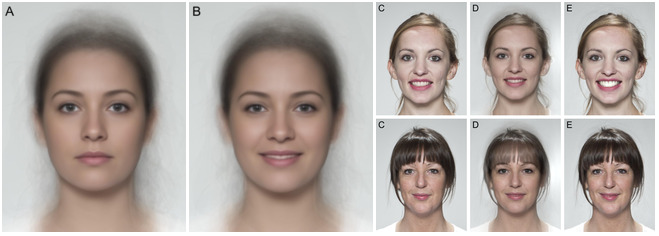
\includegraphics[width=1\linewidth]{index_files/figure-latex/transform-demo-1} \caption{Composite (A) neutral and (B) smiling faces made from 49 indvidual neutral and smiling identities. (C) Individual smiling faces were (D) averaged with the smiling composite or (E) transformed by 50\% of the shape and color differences between the neutral and smiling composites (E).}\label{fig:transform-demo}
\end{figure}

These methods were improved by wavelet-based texture averaging (Tiddeman et al., 2001), resulting in images with more realistic textural details, such as facial hair and eyebrows. This reduces the ``fuzzy'' look of composite images, but can also result in artifacts, such as lines on the forehead in Figure~\ref{fig:texture-comp}, which are a result of some images having a fringe.

\begin{figure}
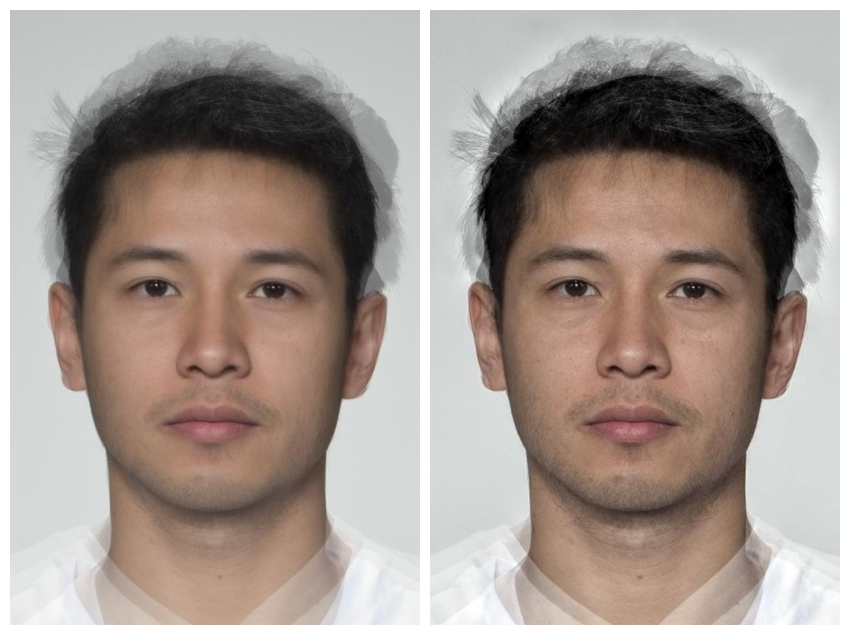
\includegraphics[width=1\linewidth]{index_files/figure-latex/texture-comp-1} \caption{Untextured and textured prototypes of 4 male faces.}\label{fig:texture-comp}
\end{figure}

The desktop version of Psychomorph was last updated in 2013, and can be difficult to install on some computers. To solve this problem, we started developing WebMorph (L. M. DeBruine, 2018), a web-based version that uses the \href{https://users.aber.ac.uk/bpt/jpsychomorph/version6/javadoc/}{Facemorph Java package} from Psychomorph for averaging and transforming images, but has independent methods for delineation and batch processing. While the desktop version of Psychomorph has limited batch processing ability, it requires a knowledge of Java to be fully scriptable. WebMorph has more extensive batch processing capacity, including the ability to set up image processing scripts in a spreadsheet, but some processes such as delineation still require a fair amount of manual processing. In this paper, we introduce webmorphR (L. M. DeBruine, 2022a), an R package companion to WebMorph that allows you to create R scripts to fully and reproducibly describe all of the steps of image processing and easily apply them to a new set of images.

\begin{table}

\caption{\label{tab:glossary}Glossary of terms.}
\centering
\begin{tabular}[t]{l|l}
\hline
Term & Definition\\
\hline
composite & an average of more than one face image\\
\hline
delineation & the x- and y-coordinates for a specific template that describe an image\\
\hline
landmark & a point that marks corresponding locations on different images\\
\hline
lines & connections between landmarks; these may be used to interpolate new landmarks for morphing\\
\hline
morphing & blending two or more images to make an image with an average shape andor color\\
\hline
prototype & an average of faces with similar characteristics, such as expression, gender, age, and/or ethnic group\\
\hline
template & a set of landmark points that define shape and the way these are connected with lines; only image with the same template can be averaged or transformed\\
\hline
transforming & changing the shape and/or color of an image by some proportion of a vector that is  defined as the difference between two images\\
\hline
\end{tabular}
\end{table}

\hypertarget{methods}{%
\subsection{Methods}\label{methods}}

In this section, we will cover some common image manipulations and how to achieve them reproducibly using webmorphR (L. M. DeBruine, 2022a). We will also be using webmorphR.stim (L. DeBruine \& Jones, 2017), a package that contains a number of open-source face image sets, and webmorphR.dlib (L. M. DeBruine, 2022b), a package that provides dlib models and functions for automatic face detection. These latter two packages cannot be made available on CRAN (the main repository for R packages) because of their large file size.

\hypertarget{editing}{%
\subsubsection{Editing}\label{editing}}

Almost all image sets start with raw images that need to be cropped, resized, rotated, padded, and/or color normalised. Although many reproducible methods exist to manipulate images in these ways, they are complicated when an image has an associated delineation, so webmorphR has functions that alter the image and delineation together (Fig.~\ref{fig:editing}).

\begin{Shaded}
\begin{Highlighting}[]
\NormalTok{orig }\OtherTok{\textless{}{-}} \FunctionTok{demo\_stim}\NormalTok{() }\CommentTok{\# load demo images}
\NormalTok{mirrored }\OtherTok{\textless{}{-}} \FunctionTok{mirror}\NormalTok{(orig)}
\NormalTok{cropped  }\OtherTok{\textless{}{-}} \FunctionTok{crop}\NormalTok{(orig, }\AttributeTok{width =} \FloatTok{0.75}\NormalTok{, }\AttributeTok{height =} \FloatTok{0.75}\NormalTok{)}
\NormalTok{resized  }\OtherTok{\textless{}{-}} \FunctionTok{resize}\NormalTok{(orig, }\FloatTok{0.75}\NormalTok{)}
\NormalTok{rotated  }\OtherTok{\textless{}{-}} \FunctionTok{rotate}\NormalTok{(orig, }\AttributeTok{degrees =} \DecValTok{180}\NormalTok{)}
\NormalTok{padded   }\OtherTok{\textless{}{-}} \FunctionTok{pad}\NormalTok{(orig, }\DecValTok{30}\NormalTok{, }\AttributeTok{fill =} \StringTok{"black"}\NormalTok{)}
\NormalTok{grey     }\OtherTok{\textless{}{-}} \FunctionTok{greyscale}\NormalTok{(orig)}
\end{Highlighting}
\end{Shaded}



\begin{figure}
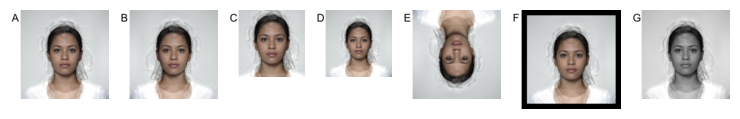
\includegraphics[width=1\linewidth]{index_files/figure-latex/editing-1} \caption{Examples of image manipulations: (A) original image, (B) mirrored, (C) cropped to 75\%, (D) resized to 75\%, (E) rotated 180 degrees, (F) 30 pixels of black padding added, and (G) greyscale.}\label{fig:editing}
\end{figure}

\hypertarget{delineation}{%
\subsubsection{Delineation}\label{delineation}}

The image manipulations above work best if your raw images start the same size and aspect ratio, with the faces in the same orientation and position on each image. This is frequently not the case with raw images. Image delineation provides a way to set image manipulation parameters relative to face landmarks by marking corresponding points according to a template.

WebMorph.org's default face template marks 189 points (Fig.~\ref{fig:delineate}). Some of these points have very clear anatomical locations, such as point 0 (``left pupil''), while others have only approximate placements and are used mainly for masking or preventing morphing artifacts from affecting the background of images, such as point 147 (``about 2cm to the left of the top of the left ear (creates oval around head)''). Template point numbering is 0-based because PsychoMorph was originally written in Java.

\begin{figure}
\includegraphics[width=1\linewidth]{index_files/figure-latex/delineate-1} \caption{Default webmorph FRL template}\label{fig:delineate}
\end{figure}

The function \texttt{tem\_def()} retrieves a template definition that includes point names, default coordinates, and the identity of the symmetrically matching point for mirroring or symmetrising images Table~\ref{tab:tem-def}.

\begin{table}

\caption{\label{tab:tem-def}The first 10 landmark points of WebMorph.org's default "FRL" template.}
\centering
\begin{tabular}[t]{r|l|r|r|r}
\hline
n & name & x & y & sym\\
\hline
0 & left pupil & 166 & 275 & 1\\
\hline
1 & right pupil & 284 & 275 & 0\\
\hline
2 & top of left iris & 165 & 267 & 10\\
\hline
3 & top-left of left iris & 156 & 270 & 17\\
\hline
4 & left of left iris & 154 & 277 & 16\\
\hline
5 & bottom-left of left iris & 157 & 283 & 15\\
\hline
6 & bottom of left iris & 166 & 286 & 14\\
\hline
7 & bottom-right of left iris & 174 & 283 & 13\\
\hline
8 & right of left iris & 177 & 276 & 12\\
\hline
9 & top-right of left iris & 175 & 270 & 11\\
\hline
\end{tabular}
\end{table}

You can automatically delineate faces with a simpler template (Fig.~\ref{fig:auto-delin}) using the online services provided through the free web platform Face++ (2021), or dlib models provided by \href{https://github.com/davisking/dlib-models}{Davis King on a CC-0 license} and included in the \texttt{webmorphR.dlib} package.

\begin{Shaded}
\begin{Highlighting}[]
\CommentTok{\# load 5 images with FRL templates}
\NormalTok{f }\OtherTok{\textless{}{-}} \FunctionTok{load\_stim\_neutral}\NormalTok{(}\StringTok{"006|038|064|066|135"}\NormalTok{)}

\CommentTok{\# remove templates and auto{-}delineate with dlib}
\CommentTok{\# requires a python installation}
\NormalTok{dlib70\_tem }\OtherTok{\textless{}{-}} \FunctionTok{auto\_delin}\NormalTok{(f, }\StringTok{"dlib70"}\NormalTok{, }\AttributeTok{replace =} \ConstantTok{TRUE}\NormalTok{)}
\NormalTok{dlib7\_tem }\OtherTok{\textless{}{-}} \FunctionTok{auto\_delin}\NormalTok{(f, }\StringTok{"dlib7"}\NormalTok{, }\AttributeTok{replace =} \ConstantTok{TRUE}\NormalTok{)}

\CommentTok{\# remove templates and auto{-}delineate with Face++}
\CommentTok{\# requires a Face++ account; see ?webmorphR::auto\_delin}
\NormalTok{fpp106\_tem }\OtherTok{\textless{}{-}} \FunctionTok{auto\_delin}\NormalTok{(f, }\StringTok{"fpp106"}\NormalTok{, }\AttributeTok{replace =} \ConstantTok{TRUE}\NormalTok{)}
\NormalTok{fpp83\_tem }\OtherTok{\textless{}{-}} \FunctionTok{auto\_delin}\NormalTok{(f, }\StringTok{"fpp83"}\NormalTok{, }\AttributeTok{replace =} \ConstantTok{TRUE}\NormalTok{)}
\end{Highlighting}
\end{Shaded}

\begin{figure}
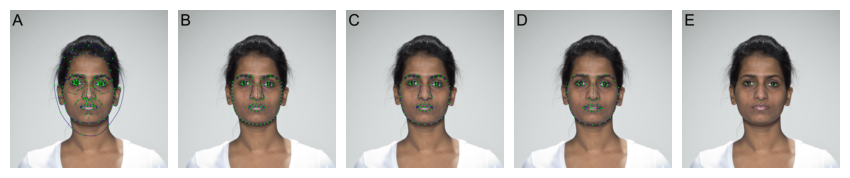
\includegraphics[width=1\linewidth]{index_files/figure-latex/auto-delin-1} \caption{Delineation templates: (A) manual delineation using the FRL template, (B) automatic delineation using the Face++ 106-point template, (C) automatic delineation using the Face++ 83-point template, (D) automatic delineation using the 70-point dlib template, and (E) automatic delineation using the 7-point dlib template.}\label{fig:auto-delin}
\end{figure}

A study comparing the accuracy of four common measures of face shape (sexual dimorphism, distinctiveness, bilateral asymmetry, and facial width to height ratio) between automatic and manual delineation concluded that automatic delineation had higher replicability and good correlations with manual delineation (A. L. Jones et al., 2021). However, around 2\% of images had noticeably inaccurate automatic delineation, which should be screened for by outlier detection and visual inspection.

You can use the \texttt{delin()} function in webmorphR to open auto-delineated images in a visual editor to fix any inaccuracies.

\begin{Shaded}
\begin{Highlighting}[]
\NormalTok{dlib7\_tem\_fixed }\OtherTok{\textless{}{-}} \FunctionTok{delin}\NormalTok{(dlib7\_tem)}
\end{Highlighting}
\end{Shaded}

\begin{figure}
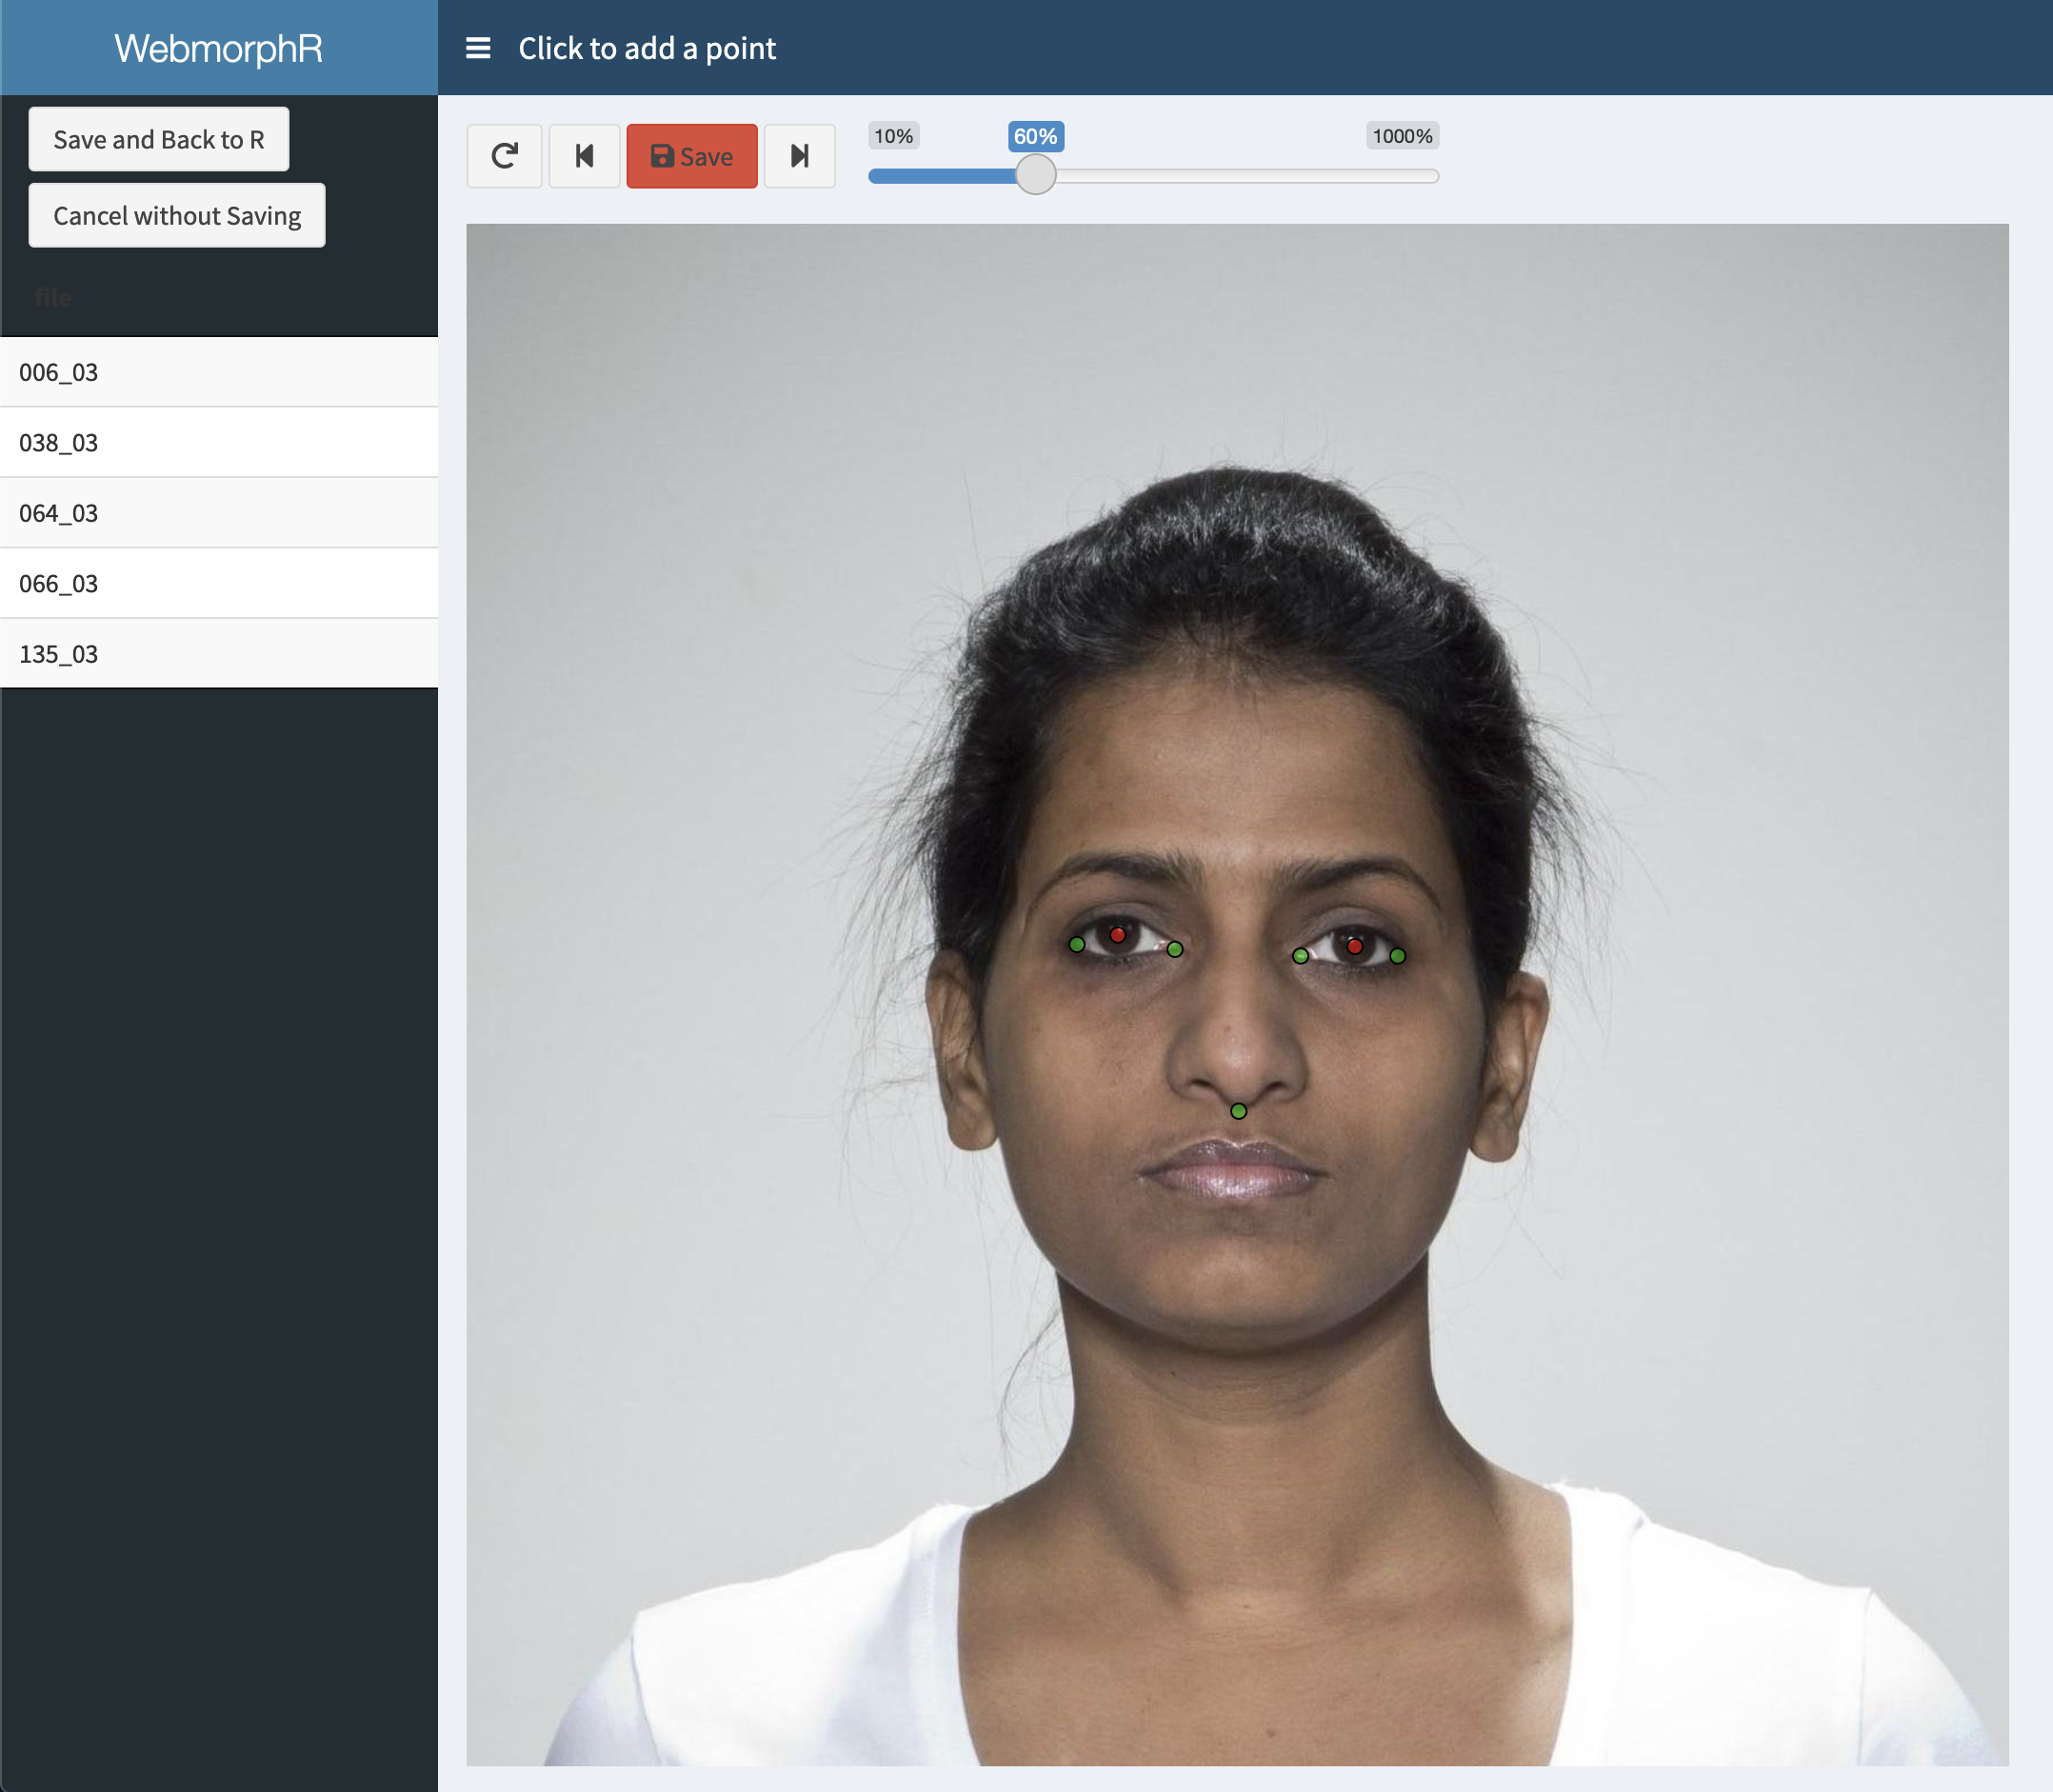
\includegraphics[width=1\linewidth]{images/delin} \caption{The shiny app interface for manual delineation adjustments.}\label{fig:delin-shiny}
\end{figure}

While automatic delineation has the advantage of being very fast and generally more replicable than manual delineation, it is more limited in the areas that can be described. Typically, automatic face detection algorithms outline the lower face shape and internal features of the face, but don't define the hairline, hair, neck, or ears. Manual delineation of these can greatly improve stimuli created through morphing or transforming (Fig.~\ref{fig:avg-comp}).

\begin{figure}
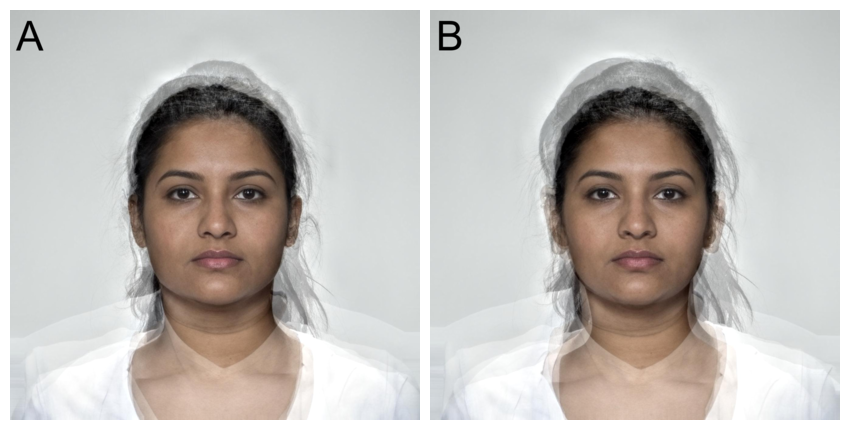
\includegraphics[width=1\linewidth]{index_files/figure-latex/avg-comp-1} \caption{Averages of 5 images made using (A) the full 189-point manual template and (B) the reduced 106-point automatic template.}\label{fig:avg-comp}
\end{figure}

\hypertarget{facial-metrics}{%
\subsubsection{Facial Metrics}\label{facial-metrics}}

Once you have images delineated, you can use the x- and y-coordinates to calculate various facial-metric measurements (Table~\ref{tab:metrics}). Get all or a subset of points with the function \texttt{get\_point()}. Remember, points are 0-based, so the first point (left pupil) is 0. This function returns a data table with one row for each point for each face.

\begin{Shaded}
\begin{Highlighting}[]
\NormalTok{eye\_points }\OtherTok{\textless{}{-}} \FunctionTok{get\_point}\NormalTok{(f, }\AttributeTok{pt =} \DecValTok{0}\SpecialCharTok{:}\DecValTok{1}\NormalTok{)}
\end{Highlighting}
\end{Shaded}

\begin{table}

\caption{\label{tab:unnamed-chunk-7}Coordinates of the first two points.}
\centering
\begin{tabular}[t]{l|r|r|r}
\hline
image & point & x & y\\
\hline
006\_03 & 0 & 570 & 620\\
\hline
006\_03 & 1 & 776 & 630\\
\hline
038\_03 & 0 & 580 & 580\\
\hline
038\_03 & 1 & 793 & 577\\
\hline
064\_03 & 0 & 570 & 578\\
\hline
064\_03 & 1 & 783 & 570\\
\hline
066\_03 & 0 & 562 & 595\\
\hline
066\_03 & 1 & 790 & 599\\
\hline
135\_03 & 0 & 573 & 639\\
\hline
135\_03 & 1 & 788 & 639\\
\hline
\end{tabular}
\end{table}

The \texttt{metrics()} function helps you quickly calculate the distance between any two points, such as the pupil centres, or use a more complicated formula, such as the face width-to-height ratio from Lefevre et al. (2013).

\begin{Shaded}
\begin{Highlighting}[]
\CommentTok{\# inter{-}pupillary distance between points 0 and 1}
\NormalTok{ipd }\OtherTok{\textless{}{-}} \FunctionTok{metrics}\NormalTok{(f, }\FunctionTok{c}\NormalTok{(}\DecValTok{0}\NormalTok{, }\DecValTok{1}\NormalTok{))}

\CommentTok{\# face width{-}to{-}height ratio}
\NormalTok{left\_cheek }\OtherTok{\textless{}{-}} \FunctionTok{metrics}\NormalTok{(f, }\StringTok{"min(x[110],x[111],x[109])"}\NormalTok{)}
\NormalTok{right\_cheek }\OtherTok{\textless{}{-}} \FunctionTok{metrics}\NormalTok{(f, }\StringTok{"max(x[113],x[112],x[114])"}\NormalTok{)}
\NormalTok{bizygomatic\_width }\OtherTok{\textless{}{-}}\NormalTok{ right\_cheek }\SpecialCharTok{{-}}\NormalTok{ left\_cheek}
\NormalTok{top\_upper\_lip }\OtherTok{\textless{}{-}} \FunctionTok{metrics}\NormalTok{(f, }\StringTok{"y[90]"}\NormalTok{)}
\NormalTok{highest\_eyelid }\OtherTok{\textless{}{-}} \FunctionTok{metrics}\NormalTok{(f, }\StringTok{"min(y[20],y[25])"}\NormalTok{)}
\NormalTok{face\_height }\OtherTok{\textless{}{-}}\NormalTok{ top\_upper\_lip }\SpecialCharTok{{-}}\NormalTok{ highest\_eyelid}
\NormalTok{fwh }\OtherTok{\textless{}{-}}\NormalTok{ bizygomatic\_width}\SpecialCharTok{/}\NormalTok{face\_height}

\CommentTok{\# alternatively, do all calculations in one equation}
\NormalTok{fwh }\OtherTok{\textless{}{-}} \FunctionTok{metrics}\NormalTok{(f, }\StringTok{"abs(max(x[113],x[112],x[114]){-}min(x[110],x[111],x[109]))/abs(y[90]{-}min(y[20],y[25]))"}\NormalTok{)}
\end{Highlighting}
\end{Shaded}

\begin{table}

\caption{\label{tab:metrics}Facial metric measurements.}
\centering
\begin{tabular}[t]{l|r|r|r|r|r|r}
\hline
face & x0 & y0 & x1 & y1 & ipd & fwh\\
\hline
006\_03 & 570 & 620 & 776 & 630 & 206.2426 & 2.218905\\
\hline
038\_03 & 580 & 580 & 793 & 577 & 213.0211 & 2.636580\\
\hline
064\_03 & 570 & 578 & 783 & 570 & 213.1502 & 2.351220\\
\hline
066\_03 & 562 & 595 & 790 & 599 & 228.0351 & 2.281818\\
\hline
135\_03 & 573 & 639 & 788 & 639 & 215.0000 & 2.280788\\
\hline
\end{tabular}
\end{table}

While it is \emph{possible} to calculate metrics such as width-to-height ratio from 2D face images, this does not mean it is a good idea. Even on highly standardized images, head tilt can have large effects on such measurements (Hehman et al., 2013). When image qualities such as camera type and head-to-camera distance are not standardized, facial metrics are meaningless at best (Trebicky et al., 2016).

\hypertarget{alignment}{%
\subsubsection{Alignment}\label{alignment}}

If your image set isn't highly standardised, you probably want to crop, resize and rotate your images to get them all in approximately the same orientation on images of the same size. There are several reproducible options, each with pros and cons.

One-point alignment (Fig.~\ref{fig:norm-comp}A) doesn't rotate or resize the image at all, but aligns one of the delineation points across images. This is ideal when you know that your camera-to-head distance and orientation was standard (or meaningfully different) across images and you want to preserve this in the stimuli, but you still need to get them all in the same position and image size.

Two-point alignment (Fig.~\ref{fig:norm-comp}B) resizes and rotates the images so that two points (usually the centres of the eyes) are in the same position on each image. This will alter relative head size such that people with very close-set eyes will appear to have larger heads than people with very wide-set eyes. This technique is good for getting images into the same orientation when you didn't have any control over image rotation and camera-to-head distance of the original photos.

Procrustes alignment (Fig.~\ref{fig:norm-comp}C) resizes and rotates the images so that each delineation point is as aligned as possible across all images. This can obscure meaningful differences in relative face size (e.g., a baby's face will be as large as an adult's), but can be superior to two-point alignment. While this requires that the whole face be delineated, you can use a minimal template such as a face outline or the Face++ auto-delineation to achieve good results.

You can very quickly delineate an image set with a custom template using the \texttt{delin()} function in webmorphR if auto-delineation doesn't provide suitable points.

\begin{Shaded}
\begin{Highlighting}[]
\CommentTok{\# one{-}point alignment}
\NormalTok{onept }\OtherTok{\textless{}{-}} \FunctionTok{align}\NormalTok{(f, }\AttributeTok{pt1 =} \DecValTok{55}\NormalTok{, }\AttributeTok{pt2 =} \DecValTok{55}\NormalTok{,}
               \AttributeTok{x1 =} \FunctionTok{width}\NormalTok{(f)}\SpecialCharTok{/}\DecValTok{2}\NormalTok{, }\AttributeTok{y1 =} \FunctionTok{height}\NormalTok{(f)}\SpecialCharTok{/}\DecValTok{2}\NormalTok{,}
               \AttributeTok{fill =} \StringTok{"dodgerblue"}\NormalTok{)}

\CommentTok{\# two{-}point alignment}
\NormalTok{twopt }\OtherTok{\textless{}{-}} \FunctionTok{align}\NormalTok{(f, }\AttributeTok{pt1 =} \DecValTok{0}\NormalTok{, }\AttributeTok{pt2 =} \DecValTok{1}\NormalTok{, }\AttributeTok{fill =} \StringTok{"dodgerblue"}\NormalTok{)}

\CommentTok{\# procrustes alignment}
\NormalTok{proc }\OtherTok{\textless{}{-}} \FunctionTok{align}\NormalTok{(f, }\AttributeTok{pt1 =} \DecValTok{0}\NormalTok{, }\AttributeTok{pt2 =} \DecValTok{1}\NormalTok{, }\AttributeTok{procrustes =} \ConstantTok{TRUE}\NormalTok{, }\AttributeTok{fill =} \StringTok{"dodgerblue"}\NormalTok{)}
\end{Highlighting}
\end{Shaded}

\begin{figure}
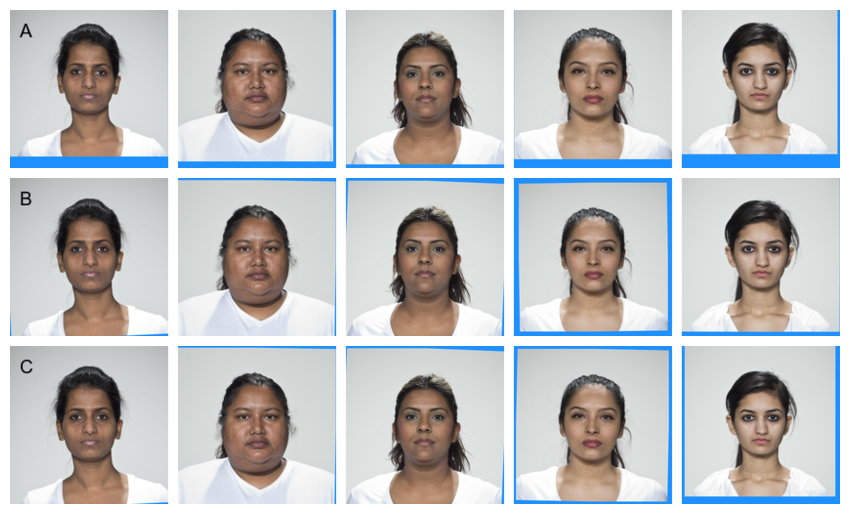
\includegraphics[width=1\linewidth]{index_files/figure-latex/norm-comp-1} \caption{Original images with different alignments. (A) One-point alignment placing the bottom of the nose point in the centre of the image. (B) Two-point alignment placing the eye centre points in the same position as the average image. (C) Procrustes alignment moved, rotated, and resized all images to most closely match the average face. A blue background was used to highlight the difference here, but normally a colour matching the image background would be used or the images would be cropped.}\label{fig:norm-comp}
\end{figure}

\hypertarget{masking}{%
\subsubsection{Masking}\label{masking}}

Oftentimes, researchers will want to remove the background, hair, and clothing from an image to avoid confounds. For example, the presence versus absence of hairstyle information can reverse preferences for masculine versus feminine male averages (L. M. DeBruine et al., 2006).

The ``standard oval mask'' has enjoyed widespread popularity because it is straightforward to add to images using programs like PhotoShop. WebmorphR's \texttt{mask\_oval()} function allows you to set oval boundaries manually (Fig.~\ref{fig:mask}A) or in relation to minimum and maximum template coordinates for each face (Fig.~\ref{fig:mask}B) or across the full image set. An arguably better way to mask out hair, clothing and background from images is to crop around the curves defined by the template (Fig.~\ref{fig:mask}C).

\begin{Shaded}
\begin{Highlighting}[]
\CommentTok{\# standard oval mask}
\NormalTok{bounds }\OtherTok{\textless{}{-}} \FunctionTok{list}\NormalTok{(}\AttributeTok{t =} \DecValTok{200}\NormalTok{, }\AttributeTok{r =} \DecValTok{400}\NormalTok{, }\AttributeTok{b =} \DecValTok{300}\NormalTok{, }\AttributeTok{l =} \DecValTok{400}\NormalTok{)}
\NormalTok{oval }\OtherTok{\textless{}{-}} \FunctionTok{mask\_oval}\NormalTok{(f, bounds, }\AttributeTok{fill =} \StringTok{"dodgerblue"}\NormalTok{)}

\CommentTok{\# template{-}aware oval mask}
\NormalTok{oval\_tem }\OtherTok{\textless{}{-}}\NormalTok{ f }\SpecialCharTok{|}\ErrorTok{\textgreater{}}
  \FunctionTok{subset\_tem}\NormalTok{(}\FunctionTok{features}\NormalTok{(}\StringTok{"gmm"}\NormalTok{)) }\SpecialCharTok{|}\ErrorTok{\textgreater{}} \CommentTok{\# remove external points}
  \FunctionTok{mask\_oval}\NormalTok{(}\AttributeTok{fill =} \StringTok{"dodgerblue"}\NormalTok{) }\CommentTok{\# oval boundaries to max and min template points}

\CommentTok{\# template{-}aware mask}
\NormalTok{masked }\OtherTok{\textless{}{-}} \FunctionTok{mask}\NormalTok{(f, }\FunctionTok{c}\NormalTok{(}\StringTok{"face"}\NormalTok{, }\StringTok{"neck"}\NormalTok{, }\StringTok{"ears"}\NormalTok{), }\AttributeTok{fill =} \StringTok{"dodgerblue"}\NormalTok{)}
\end{Highlighting}
\end{Shaded}

\begin{figure}
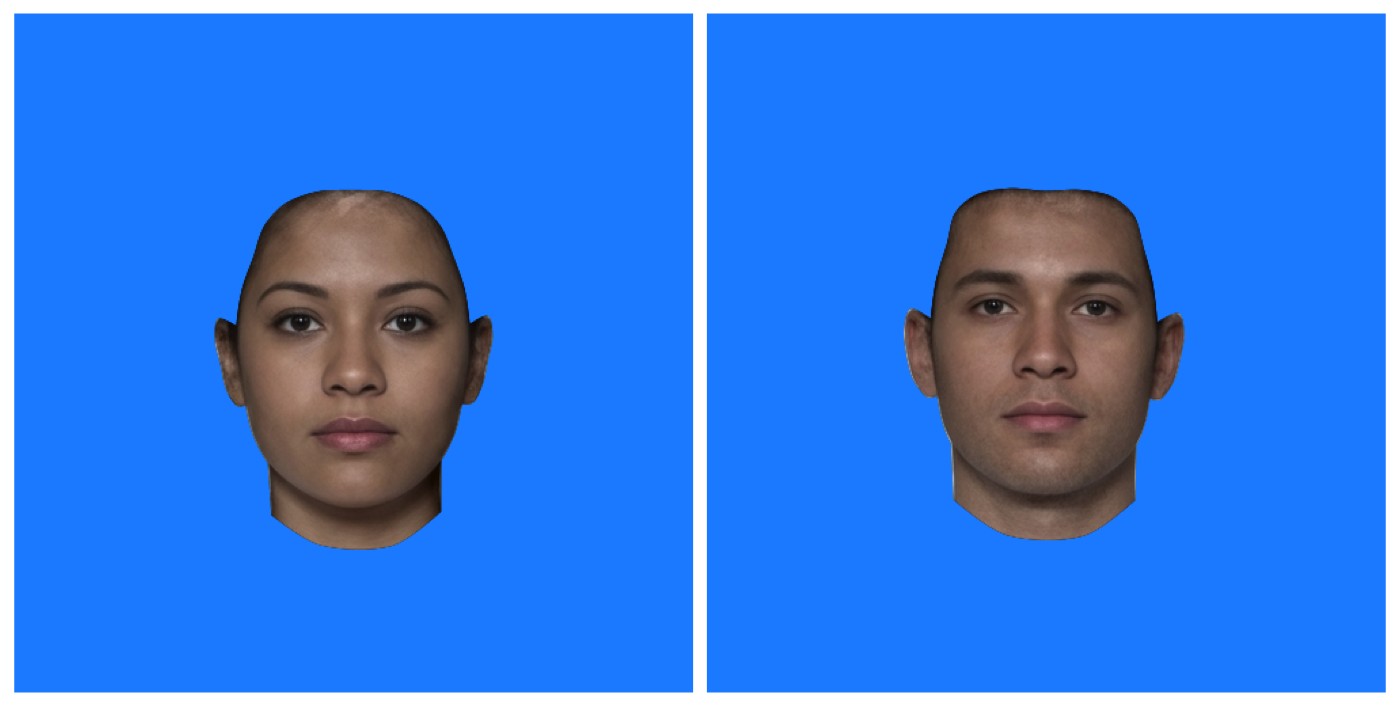
\includegraphics[width=1\linewidth]{index_files/figure-latex/mask-1} \caption{Images masked with (A) an oval defined by image coordinates, (B) an oval defined by the minimum and maximum x- and y-coordinates of template points, or (C) to include face, ears and neck.}\label{fig:mask}
\end{figure}

\hypertarget{averaging}{%
\subsubsection{Averaging}\label{averaging}}

Creating average images (also called composite or prototype images) through morphing can be a way to visualise the differences between groups (Burton et al., 2005), manipulate averageness (Little et al., 2011), or create prototypical faces for image transformations.

Averaging faces with texture (Tiddeman et al., 2005, 2001) makes composite images look more realistic (Fig.~\ref{fig:avg-texture}A). However, averages created without texture averaging look smoother and may be more appropriate for transforming color (Fig.~\ref{fig:avg-texture}B).

\begin{Shaded}
\begin{Highlighting}[]
\NormalTok{avg\_tex }\OtherTok{\textless{}{-}} \FunctionTok{avg}\NormalTok{(f, }\AttributeTok{texture =} \ConstantTok{TRUE}\NormalTok{)}
\NormalTok{avg\_notex }\OtherTok{\textless{}{-}} \FunctionTok{avg}\NormalTok{(f, }\AttributeTok{texture =} \ConstantTok{FALSE}\NormalTok{)}
\end{Highlighting}
\end{Shaded}

\begin{figure}
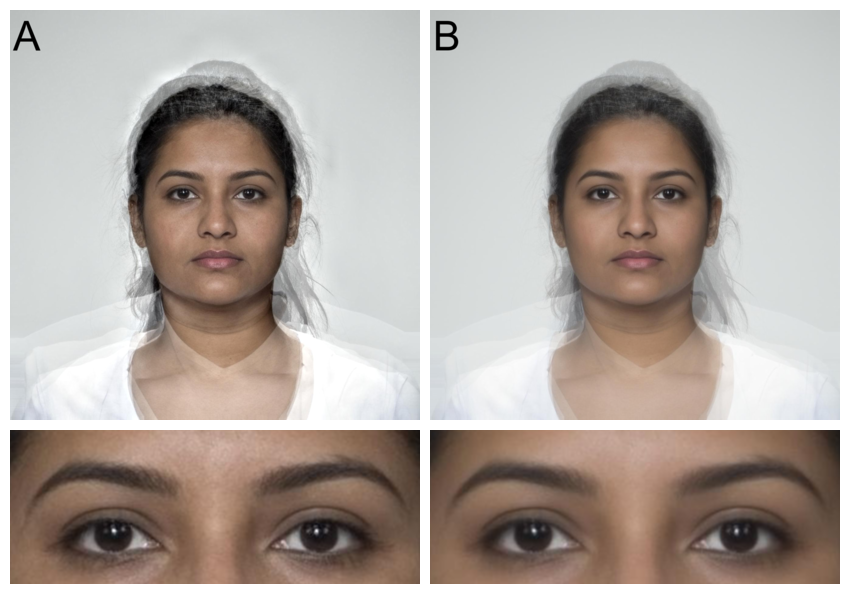
\includegraphics[width=1\linewidth]{index_files/figure-latex/avg-texture-1} \caption{An average of 5 faces created (A) with texture averaging and (B) without.}\label{fig:avg-texture}
\end{figure}

\hypertarget{transforming}{%
\subsubsection{Transforming}\label{transforming}}

Transforming alters the appearance of one face by some proportion of the differences between two other faces. This technique is distinct from morphing. For example, you can transform a face in the dimension of sexual dimorphism by calculating the shape and color differences between a prototype female face (Fig.~\ref{fig:trans-vs-morph}A) and a prototype male face (Fig.~\ref{fig:trans-vs-morph}B). If you morph an individual female face with these images, you get faces that are halfway between the individual and prototype faces (Fig.~\ref{fig:trans-vs-morph}C,D). However, if you transform the individual face by 50\% of the prototype differences, you get feminised and masculinized versions of the individual face (Fig.~\ref{fig:trans-vs-morph}E,F).

\begin{figure}
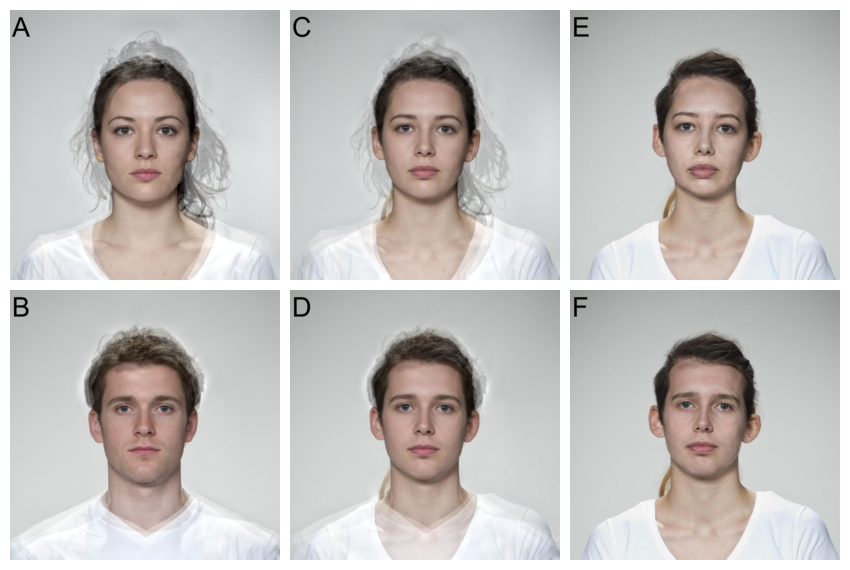
\includegraphics[width=0.75\linewidth]{index_files/figure-latex/trans-vs-morph-1} \caption{Morphing versus transforming: (A) female and male composite images, (B) averages of the composites with the individual image, (C) transforms of the individual image along the male-female continuum.}\label{fig:trans-vs-morph}
\end{figure}

If, for example, the individual female face was more feminine than the average female face, morphing with the average female face produces an image that is \emph{less} feminine than the original individual, while transforming along the male-female dimension produces and image that is always \emph{more} feminine than the original. Morphing with a prototype also results in an image with increased averageness, while transforming maintains individually distinctive features.

Transforming also allows you to manipulate shape and colour independently (Fig.~\ref{fig:trans-shape-color}).

\begin{figure}
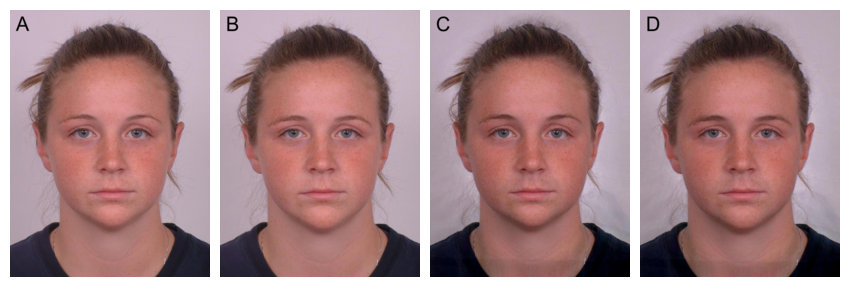
\includegraphics[width=1\linewidth]{index_files/figure-latex/trans-shape-color-1} \caption{Transforming shape and color independently: (A) original individual image, (B) shape only, (C), color only, (D) both shape and color.}\label{fig:trans-shape-color}
\end{figure}

\hypertarget{symmetrising}{%
\subsubsection{Symmetrising}\label{symmetrising}}

Although a common technique (e.g., Mealey et al., 1999), left-left and right-right mirroring (Fig.~\ref{fig:mirror-sym}) is not recommended for investigating perceptions of facial symmetry. This is because this method typically produces unnatural images for any face that isn't already perfectly symmetric. For example, if the nose does not lie in a perfectly straight line from the centre point between the eyes to the centre of the mouth, then one of the mirrored halves will have a much wider nose than the original face, while the the other half will have a much narrower nose than the original face. In extreme cases, one mirrored version can end up with three nostrils and the other with a single nostril.

\begin{figure}
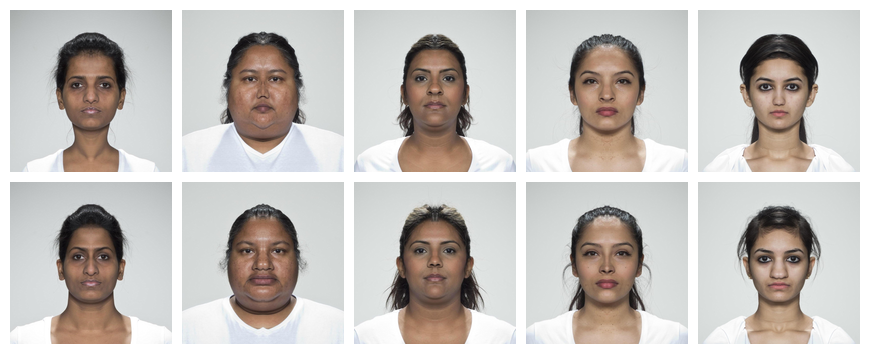
\includegraphics[width=1\linewidth]{index_files/figure-latex/mirror-sym-1} \caption{Left-left (top) and right-right (bottom) mirrored images. The code for making these images is in the supplemental materials, but we only recommend using this method to demonstrate how misleading it is.}\label{fig:mirror-sym}
\end{figure}

A morph-based technique is a more realistic way to manipulate symmetry Paukner et al. (2017). It preserves the individual's characteristic feature shapes and avoids the problem of having to choose an axis of symmetry on a face that isn't perfectly symmetrical. In this method, the original face is mirror-reversed and each template point is re-labelled. The original and mirrored images are averaged together to create a perfectly symmetric version of the image that has the same feature widths as the original face (Fig.~\ref{fig:morph-sym}). You can also use this symmetric version to create asymmetric versions of the original face through transforming: exaggerating the differences between the original and the symmetric version.

\begin{Shaded}
\begin{Highlighting}[]
\NormalTok{sym\_both }\OtherTok{\textless{}{-}} \FunctionTok{symmetrize}\NormalTok{(f)}
\NormalTok{sym\_shape }\OtherTok{\textless{}{-}} \FunctionTok{symmetrize}\NormalTok{(f, }\AttributeTok{color =} \DecValTok{0}\NormalTok{)}
\NormalTok{sym\_color }\OtherTok{\textless{}{-}} \FunctionTok{symmetrize}\NormalTok{(f, }\AttributeTok{shape =} \DecValTok{0}\NormalTok{)}
\NormalTok{sym\_anti }\OtherTok{\textless{}{-}} \FunctionTok{symmetrize}\NormalTok{(f, }\AttributeTok{shape =} \SpecialCharTok{{-}}\FloatTok{1.0}\NormalTok{, }\AttributeTok{color =} \DecValTok{0}\NormalTok{)}
\end{Highlighting}
\end{Shaded}

\begin{figure}
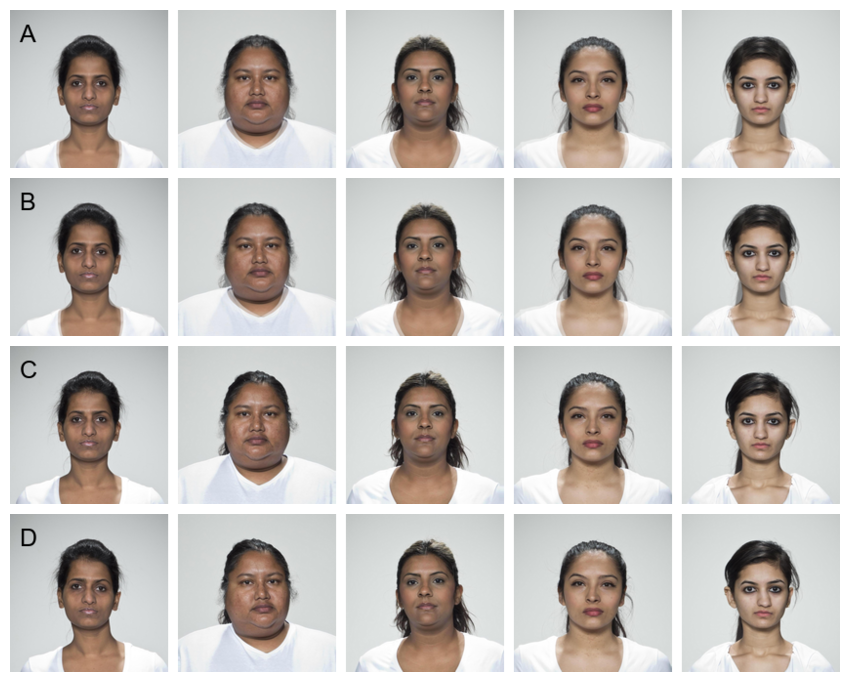
\includegraphics[width=1\linewidth]{index_files/figure-latex/morph-sym-1} \caption{Images with different types of symmetry: (A) symmetric shape and color, (B) symmetric color, (C) symmetric shape, (D) asymmetric shape.}\label{fig:morph-sym}
\end{figure}

\hypertarget{case-studies}{%
\subsection{Case Studies}\label{case-studies}}

In this section, we will demonstrate how more complex face image manipulations can be scripted, such as the creation of prototype faces, making emotion continuua, manipulating sexual dimorphism, manipulating resemblance, and labelling stimuli with words or images.

\hypertarget{london-face-set}{%
\subsubsection{London Face Set}\label{london-face-set}}

We will use the open-source, CC-BY licensed image set, the Face Research Lab London Set (L. M. DeBruine \& Jones, 2017b). Images are of 102 adults whose pictures were taken in London, UK, in April 2012 for a project with Nikon camera (Fig.~\ref{fig:london-set}). All individuals were paid and gave signed consent for their images to be ``used in lab-based and web-based studies in their original or altered forms and to illustrate research (e.g., in scientific journals, news media or presentations).''

\begin{figure}
\includegraphics[width=1\linewidth]{index_files/figure-latex/london-set-1} \caption{The 102 neutral front faces in the London Face Set.}\label{fig:london-set}
\end{figure}

Each subject has one smiling and one neutral pose. For each pose, 5 full colour images were simultaneously taken from different angles: left profile, left three-quarter, front, right three-quarter, and right profile, but we will only use the front-facing images in the examples below. These images were cropped to 1350x1350 pixels and the faces were manually centered (many years ago before we made the tools in this paper). The neutral front images have template files that mark out 189 coordinates delineating face shape for use with Psychomorph or WebMorph.

\hypertarget{protoypes}{%
\subsubsection{Protoypes}\label{protoypes}}

The first step for many types of stimuli is to create prototype faces for some categories, such as expression or gender. The faces that make up these averages should be matched for other characteristics that you want to avoid confounding with the categories of interest, such as age or ethnicity. Here, we will choose 5 Black female faces, automatically delineate them, align the images, and create neutral and smiling prototypes (Fig.~\ref{fig:emo-avg}).

\begin{Shaded}
\begin{Highlighting}[]
\CommentTok{\# select the relevant images and auto{-}delineate them}
\NormalTok{neu\_orig }\OtherTok{\textless{}{-}} \FunctionTok{subset}\NormalTok{(london, face\_gender }\SpecialCharTok{==} \StringTok{"female"}\NormalTok{) }\SpecialCharTok{|}\ErrorTok{\textgreater{}} 
  \FunctionTok{subset}\NormalTok{(face\_eth }\SpecialCharTok{==} \StringTok{"black"}\NormalTok{) }\SpecialCharTok{|}\ErrorTok{\textgreater{}} \FunctionTok{subset}\NormalTok{(}\DecValTok{1}\SpecialCharTok{:}\DecValTok{5}\NormalTok{) }\SpecialCharTok{|}\ErrorTok{\textgreater{}}
  \FunctionTok{auto\_delin}\NormalTok{(}\StringTok{"dlib70"}\NormalTok{, }\AttributeTok{replace =} \ConstantTok{TRUE}\NormalTok{)}

\NormalTok{smi\_orig }\OtherTok{\textless{}{-}} \FunctionTok{subset}\NormalTok{(smiling, face\_gender }\SpecialCharTok{==} \StringTok{"female"}\NormalTok{) }\SpecialCharTok{|}\ErrorTok{\textgreater{}} 
  \FunctionTok{subset}\NormalTok{(face\_eth }\SpecialCharTok{==} \StringTok{"black"}\NormalTok{) }\SpecialCharTok{|}\ErrorTok{\textgreater{}} \FunctionTok{subset}\NormalTok{(}\DecValTok{1}\SpecialCharTok{:}\DecValTok{5}\NormalTok{) }\SpecialCharTok{|}\ErrorTok{\textgreater{}}
  \FunctionTok{auto\_delin}\NormalTok{(}\StringTok{"dlib70"}\NormalTok{, }\AttributeTok{replace =} \ConstantTok{TRUE}\NormalTok{)}

\CommentTok{\# align the images}
\NormalTok{all }\OtherTok{\textless{}{-}} \FunctionTok{c}\NormalTok{(neu\_orig, smi\_orig) }
\NormalTok{aligned }\OtherTok{\textless{}{-}}\NormalTok{ all }\SpecialCharTok{|}\ErrorTok{\textgreater{}}
  \FunctionTok{align}\NormalTok{(}\AttributeTok{procrustes =} \ConstantTok{TRUE}\NormalTok{, }\AttributeTok{fill =} \FunctionTok{patch}\NormalTok{(all)) }\SpecialCharTok{|}\ErrorTok{\textgreater{}}
  \FunctionTok{crop}\NormalTok{(.}\DecValTok{6}\NormalTok{, .}\DecValTok{8}\NormalTok{, }\AttributeTok{y\_off =} \FloatTok{0.05}\NormalTok{)}

\NormalTok{neu }\OtherTok{\textless{}{-}} \FunctionTok{subset}\NormalTok{(aligned, }\DecValTok{1}\SpecialCharTok{:}\DecValTok{5}\NormalTok{)}
\NormalTok{smi }\OtherTok{\textless{}{-}} \FunctionTok{subset}\NormalTok{(aligned, }\DecValTok{6}\SpecialCharTok{:}\DecValTok{10}\NormalTok{)}

\NormalTok{neu\_avg }\OtherTok{\textless{}{-}} \FunctionTok{avg}\NormalTok{(neu, }\AttributeTok{texture =} \ConstantTok{FALSE}\NormalTok{)}
\NormalTok{smi\_avg }\OtherTok{\textless{}{-}} \FunctionTok{avg}\NormalTok{(smi, }\AttributeTok{texture =} \ConstantTok{FALSE}\NormalTok{)}
\end{Highlighting}
\end{Shaded}

\begin{figure}
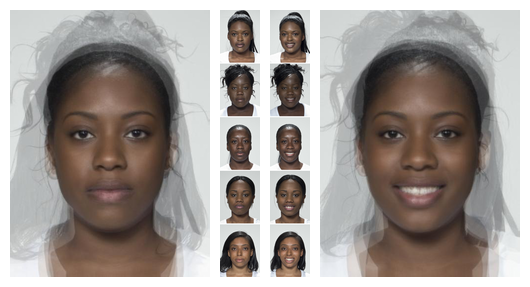
\includegraphics[width=1\linewidth]{index_files/figure-latex/emo-avg-1} \caption{Average and individual neutral and smiling faces.}\label{fig:emo-avg}
\end{figure}

We use the ``dlib70'' auto-delineation model, which is available through webmorphR.dlib (L. M. DeBruine, 2022b), but requires the installation of python and some python packages. However, it has the advantage of not requiring setting up an account at Face++ and doesn't transfer your images to a third party.

\hypertarget{emotion-continuum}{%
\subsubsection{Emotion Continuum}\label{emotion-continuum}}

Once you have two prototype images, you can set up a continuum that morphs between the images and even exaggerates beyond them (Fig.~\ref{fig:continuum}). Note that some exaggerations beyond the prototypes can produce impossible shape configurations, such as the negative smile, where the open lips from a smile go to closed at 0\% and pass through each other at negative values.

\begin{Shaded}
\begin{Highlighting}[]
\NormalTok{steps }\OtherTok{\textless{}{-}} \FunctionTok{continuum}\NormalTok{(neu\_avg, smi\_avg, }\AttributeTok{from =} \SpecialCharTok{{-}}\FloatTok{0.5}\NormalTok{, }\AttributeTok{to =} \FloatTok{1.5}\NormalTok{, }\AttributeTok{by =} \FloatTok{0.25}\NormalTok{)}
\end{Highlighting}
\end{Shaded}



\begin{figure}
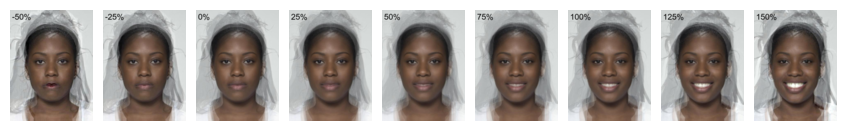
\includegraphics[width=1\linewidth]{index_files/figure-latex/continuum-1} \caption{Continuum from -50\% to +150\% smiling.}\label{fig:continuum}
\end{figure}

\hypertarget{sexual-dimorphism-transform}{%
\subsubsection{Sexual dimorphism transform}\label{sexual-dimorphism-transform}}

We can use the full templates to create sexual dimorphism transforms from neutral faces. Repeat the process above for 5 male and 5 female neutral faces, skipping the auto-delineation because these images already have webmorph templates (Fig.~\ref{fig:sexdim-avg}).

\begin{Shaded}
\begin{Highlighting}[]
\CommentTok{\# select the relevant images}
\NormalTok{f\_orig }\OtherTok{\textless{}{-}} \FunctionTok{subset}\NormalTok{(london, face\_gender }\SpecialCharTok{==} \StringTok{"female"}\NormalTok{) }\SpecialCharTok{|}\ErrorTok{\textgreater{}} 
  \FunctionTok{subset}\NormalTok{(face\_eth }\SpecialCharTok{==} \StringTok{"black"}\NormalTok{) }\SpecialCharTok{|}\ErrorTok{\textgreater{}} \FunctionTok{subset}\NormalTok{(}\DecValTok{1}\SpecialCharTok{:}\DecValTok{5}\NormalTok{)}

\NormalTok{m\_orig }\OtherTok{\textless{}{-}} \FunctionTok{subset}\NormalTok{(london, face\_gender }\SpecialCharTok{==} \StringTok{"male"}\NormalTok{) }\SpecialCharTok{|}\ErrorTok{\textgreater{}} 
  \FunctionTok{subset}\NormalTok{(face\_eth }\SpecialCharTok{==} \StringTok{"black"}\NormalTok{) }\SpecialCharTok{|}\ErrorTok{\textgreater{}} \FunctionTok{subset}\NormalTok{(}\DecValTok{1}\SpecialCharTok{:}\DecValTok{5}\NormalTok{)}

\CommentTok{\# align the images}
\NormalTok{all }\OtherTok{\textless{}{-}} \FunctionTok{c}\NormalTok{(f\_orig, m\_orig) }
\NormalTok{aligned }\OtherTok{\textless{}{-}}\NormalTok{ all }\SpecialCharTok{|}\ErrorTok{\textgreater{}}
  \FunctionTok{align}\NormalTok{(}\AttributeTok{procrustes =} \ConstantTok{TRUE}\NormalTok{, }\AttributeTok{fill =} \FunctionTok{patch}\NormalTok{(all)) }\SpecialCharTok{|}\ErrorTok{\textgreater{}}
  \FunctionTok{crop}\NormalTok{(.}\DecValTok{6}\NormalTok{, .}\DecValTok{8}\NormalTok{, }\AttributeTok{y\_off =} \FloatTok{0.05}\NormalTok{)}

\NormalTok{f }\OtherTok{\textless{}{-}} \FunctionTok{subset}\NormalTok{(aligned, }\DecValTok{1}\SpecialCharTok{:}\DecValTok{5}\NormalTok{)}
\NormalTok{m }\OtherTok{\textless{}{-}} \FunctionTok{subset}\NormalTok{(aligned, }\DecValTok{6}\SpecialCharTok{:}\DecValTok{10}\NormalTok{)}

\NormalTok{f\_avg }\OtherTok{\textless{}{-}} \FunctionTok{avg}\NormalTok{(f, }\AttributeTok{texture =} \ConstantTok{FALSE}\NormalTok{)}
\NormalTok{m\_avg }\OtherTok{\textless{}{-}} \FunctionTok{avg}\NormalTok{(m, }\AttributeTok{texture =} \ConstantTok{FALSE}\NormalTok{)}
\end{Highlighting}
\end{Shaded}

\begin{figure}
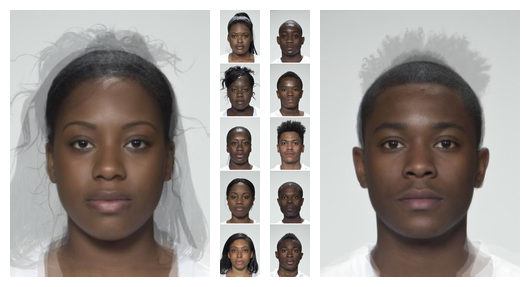
\includegraphics[width=1\linewidth]{index_files/figure-latex/sexdim-avg-1} \caption{Average and individual female and male faces.}\label{fig:sexdim-avg}
\end{figure}

Next, transform each individual image using the average female and male faces as transform endpoints (Fig.~\ref{fig:sexdim-transform}).

\begin{Shaded}
\begin{Highlighting}[]
\CommentTok{\# use a named vector for shape to automatically rename the images}
\NormalTok{sexdim }\OtherTok{\textless{}{-}} \FunctionTok{trans}\NormalTok{(}
  \AttributeTok{trans\_img =} \FunctionTok{c}\NormalTok{(f, m),}
  \AttributeTok{from\_img =}\NormalTok{ f\_avg,}
  \AttributeTok{to\_img =}\NormalTok{ m\_avg,}
  \AttributeTok{shape =} \FunctionTok{c}\NormalTok{(}\AttributeTok{fem =} \SpecialCharTok{{-}}\NormalTok{.}\DecValTok{5}\NormalTok{, }\AttributeTok{masc =}\NormalTok{ .}\DecValTok{5}\NormalTok{)}
\NormalTok{)}
\end{Highlighting}
\end{Shaded}



\begin{figure}
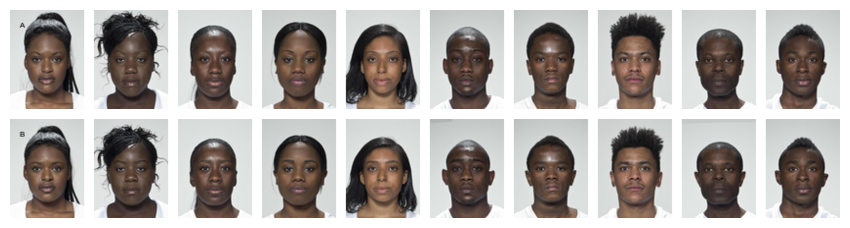
\includegraphics[width=1\linewidth]{index_files/figure-latex/sexdim-transform-1} \caption{Versions of individual faces with (A) 50\% feminised shape and (B) 50\% masculinized shape.}\label{fig:sexdim-transform}
\end{figure}

\hypertarget{self-resemblance-transform}{%
\subsubsection{Self-resemblance transform}\label{self-resemblance-transform}}

Some research involves creating ``virtual siblings'' for participants to test how they perceive and behave towards strangers with phenotypic kinship cues (L. M. DeBruine, 2004, 2005; L. M. DeBruine et al., 2011). As discussed in detail in DeBruine et al. (2008), while morphing techniques are sufficient to create same-gender virtual siblings, transforming techniques are required to make other-gender virtual siblings without confounding self-resemblance with androgyny (Fig.~\ref{fig:virtual-sibs}).

\begin{Shaded}
\begin{Highlighting}[]
\NormalTok{virtual\_sis }\OtherTok{\textless{}{-}} \FunctionTok{trans}\NormalTok{(}
  \AttributeTok{trans\_img =}\NormalTok{ f\_avg,   }\CommentTok{\# transform an average female face}
  \AttributeTok{shape =} \FloatTok{0.5}\NormalTok{,         }\CommentTok{\# by 50\% of the shape differences}
  \AttributeTok{from\_img =}\NormalTok{ m\_avg,    }\CommentTok{\# between an average male face}
  \AttributeTok{to\_img =}\NormalTok{ m) }\SpecialCharTok{|}\ErrorTok{\textgreater{}}       \CommentTok{\# and individual male faces}
  \FunctionTok{mask}\NormalTok{(}\FunctionTok{c}\NormalTok{(}\StringTok{"face"}\NormalTok{, }\StringTok{"neck"}\NormalTok{,}\StringTok{"ears"}\NormalTok{)) }

\NormalTok{virtual\_bro }\OtherTok{\textless{}{-}} \FunctionTok{trans}\NormalTok{(}
  \AttributeTok{trans\_img =}\NormalTok{ m\_avg,   }\CommentTok{\# transform an average male face}
  \AttributeTok{shape =} \FloatTok{0.5}\NormalTok{,         }\CommentTok{\# by 50\% of the shape differences}
  \AttributeTok{from\_img =}\NormalTok{ m\_avg,    }\CommentTok{\# between an average male face}
  \AttributeTok{to\_img =}\NormalTok{ m) }\SpecialCharTok{|}\ErrorTok{\textgreater{}}       \CommentTok{\# and individual male faces}
  \FunctionTok{mask}\NormalTok{(}\FunctionTok{c}\NormalTok{(}\StringTok{"face"}\NormalTok{, }\StringTok{"neck"}\NormalTok{,}\StringTok{"ears"}\NormalTok{))}
\end{Highlighting}
\end{Shaded}

\begin{figure}
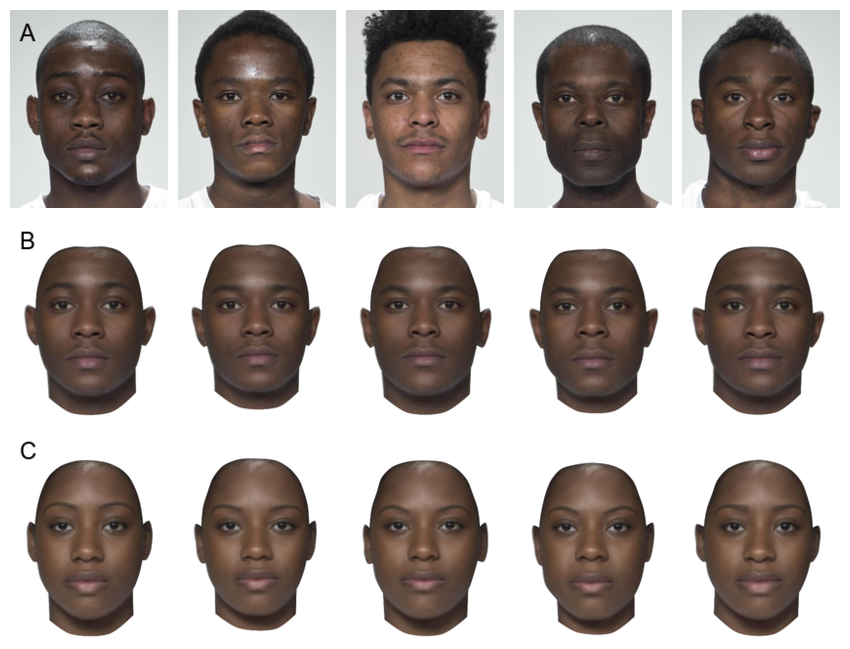
\includegraphics[width=1\linewidth]{index_files/figure-latex/virtual-sibs-1} \caption{Creating virtual siblings: (A) original images, (B) virtual brothers, (C) virtual sisters.}\label{fig:virtual-sibs}
\end{figure}

\hypertarget{labels}{%
\subsubsection{Labels}\label{labels}}

Many social perception studies require labelled images, such a minimal group designs. You can add custom labels and superimpose images on stimuli (Fig.~\ref{fig:label-comp}).

\begin{Shaded}
\begin{Highlighting}[]
\NormalTok{flags }\OtherTok{\textless{}{-}} \FunctionTok{read\_stim}\NormalTok{(}\StringTok{"images/flags"}\NormalTok{)}

\NormalTok{ingroup }\OtherTok{\textless{}{-}}\NormalTok{ f }\SpecialCharTok{|}\ErrorTok{\textgreater{}}
  \CommentTok{\# pad 10\% at the top with matching color}
  \FunctionTok{pad}\NormalTok{(}\FloatTok{0.1}\NormalTok{, }\DecValTok{0}\NormalTok{, }\DecValTok{0}\NormalTok{, }\DecValTok{0}\NormalTok{, }\AttributeTok{fill =} \FunctionTok{patch}\NormalTok{(f)) }\SpecialCharTok{|}\ErrorTok{\textgreater{}} 
  \FunctionTok{label}\NormalTok{(}\StringTok{"Scottish"}\NormalTok{, }\StringTok{"north"}\NormalTok{, }\StringTok{"+0+10"}\NormalTok{) }\SpecialCharTok{|}\ErrorTok{\textgreater{}}
  \FunctionTok{image\_func}\NormalTok{(}\StringTok{"composite"}\NormalTok{, flags}\SpecialCharTok{$}\NormalTok{saltire}\SpecialCharTok{$}\NormalTok{img, }
              \AttributeTok{gravity =} \StringTok{"northeast"}\NormalTok{, }\AttributeTok{offset =} \StringTok{"+10+10"}\NormalTok{)}

\NormalTok{outgroup }\OtherTok{\textless{}{-}}\NormalTok{ f }\SpecialCharTok{|}\ErrorTok{\textgreater{}}
  \FunctionTok{pad}\NormalTok{(}\FloatTok{0.1}\NormalTok{, }\DecValTok{0}\NormalTok{, }\DecValTok{0}\NormalTok{, }\DecValTok{0}\NormalTok{, }\AttributeTok{fill =} \FunctionTok{patch}\NormalTok{(f)) }\SpecialCharTok{|}\ErrorTok{\textgreater{}} 
  \FunctionTok{label}\NormalTok{(}\StringTok{"Welsh"}\NormalTok{, }\StringTok{"north"}\NormalTok{, }\StringTok{"+0+10"}\NormalTok{) }\SpecialCharTok{|}\ErrorTok{\textgreater{}}
  \FunctionTok{image\_func}\NormalTok{(}\StringTok{"composite"}\NormalTok{, flags}\SpecialCharTok{$}\NormalTok{ddraig}\SpecialCharTok{$}\NormalTok{img, }
             \AttributeTok{gravity =} \StringTok{"northeast"}\NormalTok{, }\AttributeTok{offset =} \StringTok{"+10+10"}\NormalTok{)}
\end{Highlighting}
\end{Shaded}

\begin{figure}
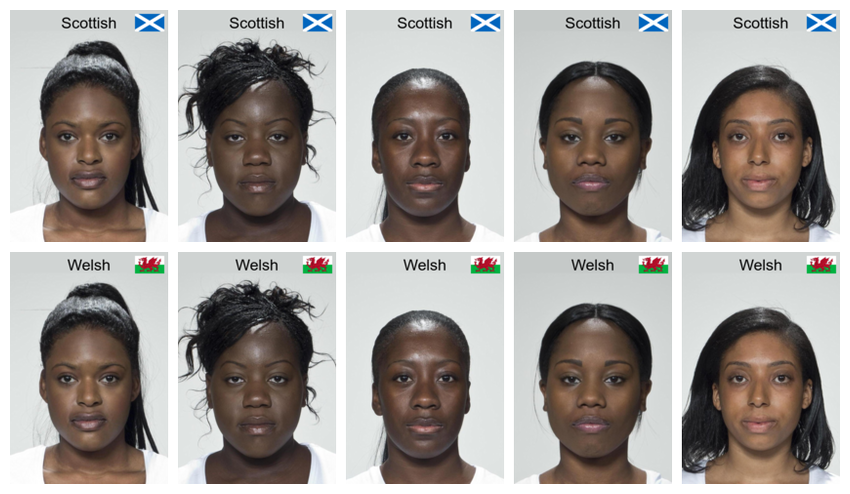
\includegraphics[width=1\linewidth]{index_files/figure-latex/label-comp-1} \caption{Stimuli with text labels and superimposed images.}\label{fig:label-comp}
\end{figure}

\hypertarget{discussion}{%
\subsection{Discussion}\label{discussion}}

Preparing your stimuli for face research in the ways described above has both personal and altruistic benefits. Once the original scripts are written, you will be able to prepare new stimuli without manual intervention. It also makes the process of changing your mind about the experimental design much less painful. If you decide that the images actually should have been aligned prior to several steps, you only need to add a line of code and rerun your script, instead of start a whole manual process over from scratch. But even more important, providing reproducible scripts can allow others to build on your work with their own images. This is beneficial for generalisability, whether or not you can share your original images.

In this section, we will discuss a number of issues related to making sure research that uses face stimuli is ethical and methodologically robust. While these issues may not be directly related to stimulus reproducibility, they are important to discuss in a paper that aims to make it easier for people to do research with face images.

\hypertarget{ethical-issues}{%
\subsubsection{Ethical Issues}\label{ethical-issues}}

Research with identifiable faces has a number of ethical issues. This means it is not always possible to share the exact images used in a study. In this case, it is all the more important for the stimulus construction methods to be clear and reproducible. However, there are other ethical issues outside of image sharing that we feel are important to highlight in a paper discussing the use of face images in research.

The use of face photographs must respect participant consent and personal data privacy. Images that are ``freely'' available on the internet, such as in Twitter profiles, are a grey area and the ethical issues should be carefully considered by the researchers and relevant ethics board.

We strongly advise against using face images in research where there is a possibility of real-world consequences for the pictured individuals. For example, do not post identifiable images of real people on real dating sites without the explicit consent of the pictured individuals for that specific research.

The use of face image analysis should never be used to predict behaviour or as automatic screening. For example, face images cannot be used to predict criminality or decide who should proceed to the interview stage in a job application. This type of application is unethical because the training data is always biased. Face image analysis can be useful for researching what aspects of face images give rise to the \emph{perception} of traits like trustworthiness, but should not be confused with the ability to detect \emph{actual} behaviour. Researchers have a responsibility to consider how their research may be misused in this manner.

\hypertarget{natural-vs-standardised-source-images}{%
\subsubsection{Natural vs standardised source images}\label{natural-vs-standardised-source-images}}

Use the right image for the question. -- Ben, do you think you could write a bit about this? I thought it would be useful to explain when/why you might use standardised images versus naturalistic ``holiday snaps''. WebmorphR can help process either, but the delineations are mainly specialised for front-facing faces (although profile face templates are available).

\begin{Shaded}
\begin{Highlighting}[]
\NormalTok{left\_profile }\OtherTok{\textless{}{-}} \FunctionTok{tem\_def}\NormalTok{(}\DecValTok{33}\NormalTok{)}
\NormalTok{right\_profile }\OtherTok{\textless{}{-}} \FunctionTok{tem\_def}\NormalTok{(}\DecValTok{32}\NormalTok{)}

\NormalTok{left\_viz }\OtherTok{\textless{}{-}} \FunctionTok{viz\_tem\_def}\NormalTok{(left\_profile)}
\NormalTok{right\_viz }\OtherTok{\textless{}{-}} \FunctionTok{viz\_tem\_def}\NormalTok{(right\_profile)}
\end{Highlighting}
\end{Shaded}

\begin{figure}
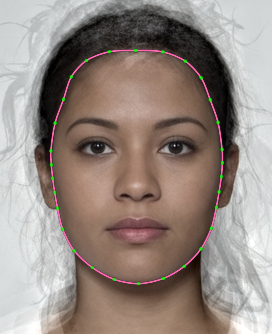
\includegraphics[width=1\linewidth]{index_files/figure-latex/unnamed-chunk-24-1} \caption{Left and right profile templates available via webmorph.org.}\label{fig:unnamed-chunk-24}
\end{figure}

\hypertarget{head-position}{%
\subsubsection{Head position}\label{head-position}}

Morphometrics -- Iris, can you add this?

\hypertarget{judging-composites}{%
\subsubsection{Judging composites}\label{judging-composites}}

In this section we will explain a serious caveat to research using composite faces that concludes something about group differences from judgements of a single pair or a small number of pairs of composites. Since we are making it easier to create composites, we do not want to inadvertently encourage research with this particular design.

As a concrete illustration, a recent paper by Alper et al. (2021) used faces from the Faceaurus database (Holtzman, 2011b). ``Holtzman (2011) standardized the assessment scores, computed average scores of self- and peer-reports, and ranked the face images based on the resulting scores. Then, prototypes for each of the personality dimensions were created by digitally combining 10 faces with the highest, and 10 faces with the lowest scores on the personality trait in question (Holtzman, 2011).'' This was done separately for male and female faces.

Since scores on the three dark triad traits are positively correlated, the three pairs of composite faces are not independent. Indeed, Holtzman states that 5 individuals were in all three low composites for the male faces, while the overlap was less extreme in other cases. With 105 observers, Holtzman found that the ability to detect the composite higher in a dark triad trait was greater than chance.

While we commend both Holtzman and Alper, Bayrak, and Yilmaz for their transparency, data sharing, and material sharing, we argue that this test has an effective N of 2, not 105, and that further replications using these images, such as those done by Alper, Bayrak, and Yilmaz, regardless of number of observers or preregistered status, lend no further weight of evidence to the assertion that dark triad traits are visible in physical appearance.

To explain this, we'll use an analogy that has nothing to do with faces (bear with us). Imagine a researcher predicts that women born on odd days are taller than women born on even days. Ridiculous, right? So let's simulate some data assuming that isn't true. The code below samples 20 women from a population with a mean height of 158.1 cm and an SD of 5.7. Half are born on odd days and half on even days.

\begin{Shaded}
\begin{Highlighting}[]
\FunctionTok{set.seed}\NormalTok{(}\DecValTok{8675309}\NormalTok{)}

\NormalTok{stim\_n }\OtherTok{\textless{}{-}} \DecValTok{10}
\NormalTok{height\_m }\OtherTok{\textless{}{-}} \FloatTok{158.1}
\NormalTok{height\_sd }\OtherTok{\textless{}{-}} \FloatTok{5.7}

\NormalTok{odd }\OtherTok{\textless{}{-}} \FunctionTok{rnorm}\NormalTok{(stim\_n, height\_m, height\_sd)}
\NormalTok{even }\OtherTok{\textless{}{-}} \FunctionTok{rnorm}\NormalTok{(stim\_n, height\_m, height\_sd)}

\FunctionTok{t.test}\NormalTok{(odd, even)}
\end{Highlighting}
\end{Shaded}

\begin{verbatim}
## 
##  Welch Two Sample t-test
## 
## data:  odd and even
## t = 1.7942, df = 17.409, p-value = 0.09016
## alternative hypothesis: true difference in means is not equal to 0
## 95 percent confidence interval:
##  -0.7673069  9.5977215
## sample estimates:
## mean of x mean of y 
##  161.1587  156.7435
\end{verbatim}

A t-test shows no significant difference, which is unsurprising. We simulated the data from the same distribution, so we know for sure there is no real difference here. Now we're going to average the height of the women with odd and even birthdays. So if we create a full-body composite of women born on odd days, she would be 161.2 cm tall, and a composite of women born on even days would be 156.7 cm tall.

If we ask 100 observers to look at these two composites, side-by-side, and judge which one looks taller, what do you imagine would happen? It's likely that nearly all of them would judge the odd-birthday composite as taller. But let's say that observers have to judge the composites independently, and they are pretty bad with height estimation, so their estimates for each composite have error with a standard deviation of 10 cm. We then compare their estimates for the odd-birthday composite with the estimate for the even-birthday composite in a paired-samples t-test.

\begin{Shaded}
\begin{Highlighting}[]
\NormalTok{obs\_n }\OtherTok{\textless{}{-}}\DecValTok{100} \CommentTok{\# number of observers}
\NormalTok{error\_sd }\OtherTok{\textless{}{-}} \DecValTok{10} \CommentTok{\# observer error}

\CommentTok{\# add the error to the composite mean heights}
\NormalTok{odd\_estimates }\OtherTok{\textless{}{-}} \FunctionTok{mean}\NormalTok{(odd) }\SpecialCharTok{+} \FunctionTok{rnorm}\NormalTok{(obs\_n, }\DecValTok{0}\NormalTok{, error\_sd)}
\NormalTok{even\_estimates }\OtherTok{\textless{}{-}} \FunctionTok{mean}\NormalTok{(even) }\SpecialCharTok{+} \FunctionTok{rnorm}\NormalTok{(obs\_n, }\DecValTok{0}\NormalTok{, error\_sd)}

\FunctionTok{t.test}\NormalTok{(odd\_estimates, even\_estimates, }\AttributeTok{paired =} \ConstantTok{TRUE}\NormalTok{)}
\end{Highlighting}
\end{Shaded}

\begin{verbatim}
## 
##  Paired t-test
## 
## data:  odd_estimates and even_estimates
## t = 3.3962, df = 99, p-value = 0.0009848
## alternative hypothesis: true mean difference is not equal to 0
## 95 percent confidence interval:
##  1.902821 7.250747
## sample estimates:
## mean difference 
##        4.576784
\end{verbatim}

Now the women with odd birthdays are significantly taller than the women with even birthdays (p = 0.00). Or are they?

We can be sure that by chance alone, our two composites will be at least slightly different on any measure, even if they are drawn from identical populations. The smaller the number of stimuli that go into each composite, the larger the mean (unsigned) size of this difference. With only 10 stimuli per composite (like the Facesaurus composites), the mean unsigned effect size of the difference between composites from populations with no real difference is 0.35 (in units of SD of the original trait distribution). If our observers are accurate enough at perceiving this difference, or we run a very large number of observers, we are virtually guaranteed to find significant results every time. Additionally, there is a 50\% chance that these results will be in the predicted direction, and this direction will be replicable across different samples of observers for the same image set.

So what does this mean for studies of the link between personality traits and facial appearance? The analogy with birth date and height holds. As long as there are facial morphologies that are even slightly consistently associated with the \emph{perception} of a trait, then composites will not be identical in that morphology. Thus, even if that morphology is totally unassociated with the trait as measured by, e.g., personality scales or peer report (which is often the case), using the composite rating method will inflate the false positive rate for concluding a difference.

The smaller the number of stimuli that go into each composite, the greater the chance that they will be visibly different in morphology related to the judgement of interest, just by chance alone. The larger the number of observers or the better observers are at detecting small differences in this morphology, the more likely that ``detection'' will be significantly above chance. Repeating this with a new set of observers does not increase the amount of evidence you have for the association between the face morphology and the measured trait. You've only measured it once in one population of faces. If observers are your unit of analyses, you are making conclusions about whether the population of observers can detect the difference between your stimuli, you cannot generalise this to new stimulus sets.

So how should researchers test for differences in facial appearance between groups? Assessment of individual face images, combined with mixed effects models (L. M. DeBruine \& Barr, 2021), can allow you to simultaneously account for variance in both observers and stimuli, avoiding the inflated false positives of the composite method (or aggregating ratings). People often use the composite method when they have too many images for any one observer to rate, but cross-classified mixed models can analyse data from counterbalanced trials or randomised subset allocation.

Another reason to use the composite rating method is when you are not ethically permitted to use individual faces in research, but are ethically permitted to use non-identifiable composite images. In this case, you can generate a large number of random composite pairs to construct the chance distribution. The equivalent to a p-value for this method is the proportion of the randomly paired composites that your target pair has a more extreme result than. While this method is too tedious to use when constructing composite faces manually, scripting allows you to automate such a task.

\begin{Shaded}
\begin{Highlighting}[]
\FunctionTok{set.seed}\NormalTok{(}\DecValTok{8675309}\NormalTok{) }\CommentTok{\# for reproducibility}

\CommentTok{\# load 20 faces}
\NormalTok{f }\OtherTok{\textless{}{-}} \FunctionTok{load\_stim\_canada}\NormalTok{(}\StringTok{"f"}\NormalTok{) }\SpecialCharTok{|}\ErrorTok{\textgreater{}} \FunctionTok{resize}\NormalTok{(}\FloatTok{0.5}\NormalTok{)}

\CommentTok{\# set to the number of random pairs you want}
\NormalTok{n\_pairs }\OtherTok{\textless{}{-}} \DecValTok{5}

\CommentTok{\# repeat this code n\_pairs times}
\NormalTok{pairs }\OtherTok{\textless{}{-}} \FunctionTok{lapply}\NormalTok{(}\DecValTok{1}\SpecialCharTok{:}\NormalTok{n\_pairs, }\ControlFlowTok{function}\NormalTok{ (i) \{}
  \CommentTok{\# sample a random 10:10 split}
\NormalTok{  rand1 }\OtherTok{\textless{}{-}} \FunctionTok{sample}\NormalTok{(}\FunctionTok{names}\NormalTok{(f), }\DecValTok{10}\NormalTok{)}
\NormalTok{  rand2 }\OtherTok{\textless{}{-}} \FunctionTok{setdiff}\NormalTok{(}\FunctionTok{names}\NormalTok{(f), rand1)}
  
  \CommentTok{\# create composite images}
\NormalTok{  comp1 }\OtherTok{\textless{}{-}} \FunctionTok{avg}\NormalTok{(f[rand1])}
\NormalTok{  comp2 }\OtherTok{\textless{}{-}} \FunctionTok{avg}\NormalTok{(f[rand2])}
  
  \CommentTok{\# save images with paired names}
\NormalTok{  nm1 }\OtherTok{\textless{}{-}} \FunctionTok{paste0}\NormalTok{(}\StringTok{"img\_"}\NormalTok{, i, }\StringTok{"\_a"}\NormalTok{)}
\NormalTok{  nm2 }\OtherTok{\textless{}{-}} \FunctionTok{paste0}\NormalTok{(}\StringTok{"img\_"}\NormalTok{, i, }\StringTok{"\_b"}\NormalTok{)}
  \FunctionTok{write\_stim}\NormalTok{(comp1, }\AttributeTok{dir =} \StringTok{"images/composites"}\NormalTok{, }\AttributeTok{names =}\NormalTok{ nm1)}
  \FunctionTok{write\_stim}\NormalTok{(comp2, }\AttributeTok{dir =} \StringTok{"images/composites"}\NormalTok{, }\AttributeTok{names =}\NormalTok{ nm2)}
\NormalTok{\})}
\end{Highlighting}
\end{Shaded}

\begin{figure}
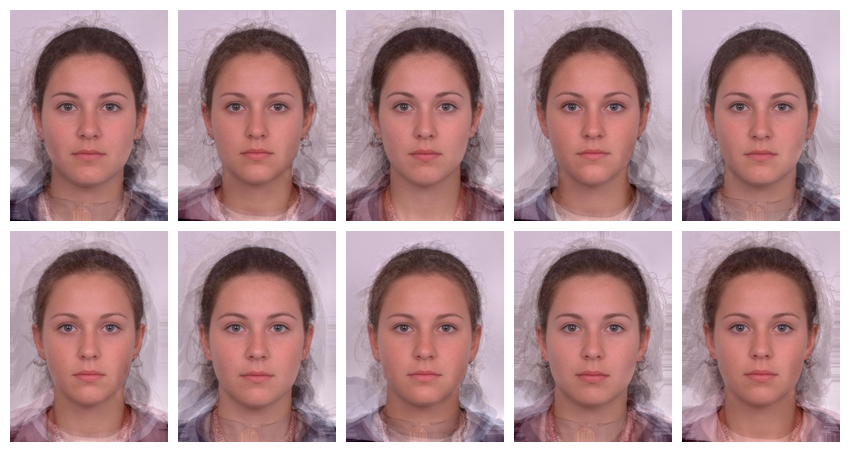
\includegraphics[width=1\linewidth]{index_files/figure-latex/rand-pair-1} \caption{Five random pairs of composites from a sample of 20 faces (10 in each composite). Can you spot any differences?}\label{fig:rand-pair}
\end{figure}

\hypertarget{open-resources}{%
\subsubsection{Open Resources}\label{open-resources}}

In conclusion, we hope that this paper has convinced you that it is both possible and desirable to use scripting to prepare stimuli for face research. You can access more detailed tutorials for webmorph.org at \url{https://debruine.github.io/webmorph/} and for webmorphR at \url{https://debruine.github.io/webmorphR/}. All image sets used in this tutorial are available on a CC-BY license at \href{https://figshare.com/search?q=webmorph\%20psychomorph}{figshare} and all software is available open source. The code to reproduce this paper can be found at \url{https://github.com/debruine/webmorphR/tree/master/paper}.

\newpage

\hypertarget{references}{%
\subsection{References}\label{references}}

We used R (Version 4.2.0; R Core Team, 2022) and the R-packages \emph{dplyr} (Version 1.0.9; Wickham et al., 2022), \emph{kableExtra} (Version 1.3.4; Zhu, 2021), \emph{magick} (Version 2.7.3; Ooms, 2021), \emph{papaja} (Version 0.1.0.9999; Aust \& Barth, 2022), \emph{tinylabels} (Version 0.2.3; Barth, 2022), \emph{webmorphR} (Version 0.1.1.9001; L. M. DeBruine, 2022a, 2022b; L. DeBruine \& Jones, 2017), \emph{webmorphR.dlib} (Version 0.0.0.9003; L. M. DeBruine, 2022b), and \emph{webmorphR.stim} (Version 0.0.0.9002; L. DeBruine \& Jones, 2017) to produce this manuscript.

\begingroup
\setlength{\parindent}{-0.5in}
\setlength{\leftskip}{0.5in}

\hypertarget{refs}{}
\begin{CSLReferences}{1}{0}
\leavevmode\vadjust pre{\hypertarget{ref-alper2021all}{}}%
Alper, S., Bayrak, F., \& Yilmaz, O. (2021). All the dark triad and some of the big five traits are visible in the face. \emph{Personality and Individual Differences}, \emph{168}, 110350. https://doi.org/\url{https://doi.org/10.1016/j.paid.2020.110350}

\leavevmode\vadjust pre{\hypertarget{ref-R-papaja}{}}%
Aust, F., \& Barth, M. (2022). \emph{{papaja}: {Prepare} reproducible {APA} journal articles with {R Markdown}}. \url{https://github.com/crsh/papaja}

\leavevmode\vadjust pre{\hypertarget{ref-barrgeneralizing}{}}%
Barr, D. J. (2007). Generalizing over encounters. In \emph{The oxford handbook of psycholinguistics}. Oxford University Press, USA.

\leavevmode\vadjust pre{\hypertarget{ref-R-tinylabels}{}}%
Barth, M. (2022). \emph{{tinylabels}: Lightweight variable labels}. \url{https://cran.r-project.org/package=tinylabels}

\leavevmode\vadjust pre{\hypertarget{ref-benson1991perception}{}}%
Benson, P. J., \& Perrett, D. I. (1991a). Perception and recognition of photographic quality facial caricatures: Implications for the recognition of natural images. \emph{European Journal of Cognitive Psychology}, \emph{3}(1), 105--135.

\leavevmode\vadjust pre{\hypertarget{ref-benson1991synthesising}{}}%
Benson, P. J., \& Perrett, D. I. (1991b). Synthesising continuous-tone caricatures. \emph{Image and Vision Computing}, \emph{9}(2), 123--129.

\leavevmode\vadjust pre{\hypertarget{ref-benson1993extracting}{}}%
Benson, P. J., \& Perrett, D. I. (1993). Extracting prototypical facial images from exemplars. \emph{Perception}, \emph{22}(3), 257--262.

\leavevmode\vadjust pre{\hypertarget{ref-burton2005robust}{}}%
Burton, A. M., Jenkins, R., Hancock, P. J., \& White, D. (2005). Robust representations for face recognition: The power of averages. \emph{Cognitive Psychology}, \emph{51}(3), 256--284.

\leavevmode\vadjust pre{\hypertarget{ref-stim-composites}{}}%
DeBruine, L. (2016). \emph{Young adult composite faces}. figshare. \url{https://doi.org/10.6084/m9.figshare.4055130.v1}

\leavevmode\vadjust pre{\hypertarget{ref-DeBruine:2007JEPHPP}{}}%
DeBruine, L. isa M., Jones, B. C., Unger, L., Little, A. C., \& Feinberg, D. R. (2007). Dissociating averageness and attractiveness: Attractive faces are not always average. \emph{Journal of Experimental Psychology: Human Perception and Performance}, \emph{33}, 1420--1430. \url{https://doi.org/10.1037/0096-1523.33.6.1420}

\leavevmode\vadjust pre{\hypertarget{ref-webmorph}{}}%
DeBruine, L. M. (2018). \emph{Webmorph: Beta release 2} (Version v0.0.0.9001) {[}Computer software{]}. Zenodo. \url{https://doi.org/10.5281/zenodo.1162670}

\leavevmode\vadjust pre{\hypertarget{ref-DeBruine_2004PRSLB}{}}%
DeBruine, L. M. (2004). Facial resemblance increases the attractiveness of same-sex faces more than other-sex faces. \emph{Proceedings of the Royal Society of London B}, \emph{271}, 2085--2090. \url{https://doi.org/10.1098/rspb.2004.2824}

\leavevmode\vadjust pre{\hypertarget{ref-DeBruine_2005PRSLB}{}}%
DeBruine, L. M. (2005). Trustworthy but not lust-worthy: Context-specific effects of facial resemblance. \emph{Proceedings of the Royal Society of London B}, \emph{272}, 919--922. \url{https://doi.org/10.1098/rspb.2004.3003}

\leavevmode\vadjust pre{\hypertarget{ref-R-webmorphR}{}}%
DeBruine, L. M. (2022a). \emph{webmorphR : Reproducible stimuli}. Zenodo. \url{https://doi.org/10.5281/zenodo.6570965}

\leavevmode\vadjust pre{\hypertarget{ref-R-webmorphR.dlib}{}}%
DeBruine, L. M. (2022b). \emph{webmorphR.dlib : Face detection for webmorphR}. \url{https://debruine.github.io/webmorphR.dlib/}

\leavevmode\vadjust pre{\hypertarget{ref-debruine2021understanding}{}}%
DeBruine, L. M., \& Barr, D. J. (2021). Understanding mixed-effects models through data simulation. \emph{Advances in Methods and Practices in Psychological Science}, \emph{4}(1), 2515245920965119.

\leavevmode\vadjust pre{\hypertarget{ref-Canada2003}{}}%
DeBruine, L. M., \& Jones, B. C. (2017a). \emph{Young adult white faces with manipulated versions}. figshare. \url{https://doi.org/10.6084/m9.figshare.4220517.v1}

\leavevmode\vadjust pre{\hypertarget{ref-FRL_London}{}}%
DeBruine, L. M., \& Jones, B. C. (2017b). \emph{Face research lab london set}. figshare. \url{https://doi.org/10.6084/m9.figshare.5047666.v5}

\leavevmode\vadjust pre{\hypertarget{ref-debruine2006correlated}{}}%
DeBruine, L. M., Jones, B. C., Little, A. C., Boothroyd, L. G., Perrett, D. I., Penton-Voak, I. S., Cooper, P. A., Penke, L., Feinberg, D. R., \& Tiddeman, B. P. (2006). Correlated preferences for facial masculinity and ideal or actual partner's masculinity. \emph{Proceedings of the Royal Society B: Biological Sciences}, \emph{273}(1592), 1355--1360.

\leavevmode\vadjust pre{\hypertarget{ref-DeBruine_2008ASB}{}}%
DeBruine, L. M., Jones, B. C., Little, A. C., \& Perrett, D. I. (2008). Social perception of facial resemblance in humans. \emph{Archives of Sexual Behavior}, \emph{37}, 64--77. \url{https://doi.org/10.1007/s10508-007-9266-0}

\leavevmode\vadjust pre{\hypertarget{ref-DeBruine_2011PNAS}{}}%
DeBruine, L. M., Jones, B. C., Watkins, C. D., Roberts, S. C., Little, A. C., Smith, F. G., \& Quist, M. (2011). Opposite-sex siblings decrease attraction, but not prosocial attributions, to self-resembling opposite-sex faces. \emph{Proceedings of the National Academy of Sciences}, \emph{108}, 11710--11714. \url{https://doi.org/10.1073/pnas.1105919108}

\leavevmode\vadjust pre{\hypertarget{ref-R-webmorphR.stim}{}}%
DeBruine, L., \& Jones, B. (2017). \emph{Face research lab london set}. figshare. \url{https://doi.org/10.6084/m9.figshare.5047666.v5}

\leavevmode\vadjust pre{\hypertarget{ref-stim-3dsk}{}}%
DeBruine, L., \& Jones, B. (2020). \emph{3DSK face set with webmorph templates}. Open Science Framework. \url{https://doi.org/10.17605/OSF.IO/A3947}

\leavevmode\vadjust pre{\hypertarget{ref-ekman1976pictures}{}}%
Ekman, P. (1976). Pictures of facial affect. \emph{Consulting Psychologists Press}.

\leavevmode\vadjust pre{\hypertarget{ref-faceplusplus}{}}%
Face++. (2021). Face++ AI open platform. In \emph{Face++}. \url{https://www.faceplusplus.com/landmarks/}

\leavevmode\vadjust pre{\hypertarget{ref-gonzalez2002digital}{}}%
Gonzalez, R. C., Woods, R. E.others. (2002). \emph{Digital image processing}. Prentice Hall Upper Saddle River, NJ. \url{https://www.pearson.com/us/higher-education/product/Gonzalez-Digital-Image-Processing-2nd-Edition/9780201180756.html}

\leavevmode\vadjust pre{\hypertarget{ref-Gronenschild_2009}{}}%
Gronenschild, E. H. B. M., Smeets, F., Vuurman, E. F. P. M., Boxtel, M. P. J. van, \& Jolles, J. (2009). The use of faces as stimuli in neuroimaging and psychological experiments: A procedure to standardize stimulus features. \emph{Behavior Research Methods}, \emph{41}, 1053--1060. \url{https://doi.org/10.3758/BRM.41.4.1053}

\leavevmode\vadjust pre{\hypertarget{ref-hehman2013enhancing}{}}%
Hehman, E., Leitner, J. B., \& Gaertner, S. L. (2013). Enhancing static facial features increases intimidation. \emph{Journal of Experimental Social Psychology}, \emph{49}(4), 747--754. \url{https://doi.org/10.1016/j.jesp.2013.02.015}

\leavevmode\vadjust pre{\hypertarget{ref-higham2016matlab}{}}%
Higham, D. J., \& Higham, N. J. (2016). \emph{MATLAB guide} (Vol. 150). Siam.

\leavevmode\vadjust pre{\hypertarget{ref-Holtzman_2011}{}}%
Holtzman, N. S. (2011a). Facing a psychopath: Detecting the dark triad from emotionally-neutral faces, using prototypes from the personality faceaurus. \emph{Journal of Research in Personality}, \emph{45}(6), 648--654.

\leavevmode\vadjust pre{\hypertarget{ref-holtzman2011facing}{}}%
Holtzman, N. S. (2011b). Facing a psychopath: Detecting the dark triad from emotionally-neutral faces, using prototypes from the personality faceaurus. \emph{Journal of Research in Personality}, \emph{45}(6), 648--654.

\leavevmode\vadjust pre{\hypertarget{ref-holzleitner2019comparing}{}}%
Holzleitner, I. J., Lee, A. J., Hahn, A. C., Kandrik, M., Bovet, J., Renoult, J. P., Simmons, D., Garrod, O., DeBruine, L. M., \& Jones, B. C. (2019). Comparing theory-driven and data-driven attractiveness models using images of real women's faces. \emph{Journal of Experimental Psychology: Human Perception and Performance}, \emph{45}(12), 1589.

\leavevmode\vadjust pre{\hypertarget{ref-jones2019biological}{}}%
Jones, A. L., \& Jaeger, B. (2019). Biological bases of beauty revisited: The effect of symmetry, averageness, and sexual dimorphism on female facial attractiveness. \emph{Symmetry}, \emph{11}(2), 279.

\leavevmode\vadjust pre{\hypertarget{ref-jones2021facial}{}}%
Jones, A. L., Schild, C., \& Jones, B. C. (2021). Facial metrics generated from manually and automatically placed image landmarks are highly correlated. \emph{Evolution and Human Behavior}, \emph{42}(3), 186--193. \url{https://doi.org/10.1016/j.evolhumbehav.2020.09.002}

\leavevmode\vadjust pre{\hypertarget{ref-jones2018no}{}}%
Jones, B. C., Hahn, A. C., Fisher, C. I., Wang, H., Kandrik, M., Lao, J., Han, C., Lee, A. J., Holzleitner, I. J., \& DeBruine, L. M. (2018). No compelling evidence that more physically attractive young adult women have higher estradiol or progesterone. \emph{Psychoneuroendocrinology}, \emph{98}, 1--5.

\leavevmode\vadjust pre{\hypertarget{ref-lefevre2013telling}{}}%
Lefevre, C. E., Lewis, G. J., Perrett, D. I., \& Penke, L. (2013). Telling facial metrics: Facial width is associated with testosterone levels in men. \emph{Evolution and Human Behavior}, \emph{34}(4), 273--279.

\leavevmode\vadjust pre{\hypertarget{ref-little2001self}{}}%
Little, A. C., Burt, D. M., Penton-Voak, I. S., \& Perrett, D. I. (2001). Self-perceived attractiveness influences human female preferences for sexual dimorphism and symmetry in male faces. \emph{Proceedings of the Royal Society of London. Series B: Biological Sciences}, \emph{268}(1462), 39--44.

\leavevmode\vadjust pre{\hypertarget{ref-Little_2011}{}}%
Little, A. C., Jones, B. C., \& DeBruine, L. M. (2011). Facial attractiveness: Evolutionary based research. \emph{Philosophical Transactions of the Royal Society B}, \emph{366}, 1638--1659. \url{https://doi.org/10.1098/rstb.2010.0404}

\leavevmode\vadjust pre{\hypertarget{ref-CFD_2015}{}}%
Ma, D. S., Correll, J., \& Wittenbrink, B. (2015). The {Chicago} face database: A free stimulus set of faces and norming data. \emph{Behavior Research Methods}, \emph{47}, 1122--1135. \url{https://doi.org/10.3758/s13428-014-0532-5}

\leavevmode\vadjust pre{\hypertarget{ref-Mealey_1999}{}}%
Mealey, L., Bridgstock, R., \& Townsend, G. C. (1999). Symmetry and perceived facial attractiveness: A monozygotic co-twin comparison. \emph{Journal of Personality and Social Psychology}, \emph{76}(1), 151.

\leavevmode\vadjust pre{\hypertarget{ref-Morrison_2018}{}}%
Morrison, D., Wang, H., Hahn, A. C., Jones, B. C., \& DeBruine, L. M. (2018). \emph{Predicting the reward value of faces and bodies from social perceptions: Supplemental materials}. OSF. \url{https://doi.org/10.17605/OSF.IO/G27WF}

\leavevmode\vadjust pre{\hypertarget{ref-nishimura2000graphicconverter}{}}%
Nishimura, D. (2000). GraphicConverter 3.9. 1. \emph{Biotech Software \& Internet Report: The Computer Software Journal for Scient}, \emph{1}(6), 267--269.

\leavevmode\vadjust pre{\hypertarget{ref-R-magick}{}}%
Ooms, J. (2021). \emph{Magick: Advanced graphics and image-processing in r}. \url{https://CRAN.R-project.org/package=magick}

\leavevmode\vadjust pre{\hypertarget{ref-paluszek2019pattern}{}}%
Paluszek, M., \& Thomas, S. (2019). Pattern recognition with deep learning. In \emph{MATLAB machine learning recipes} (pp. 209--230). Springer.

\leavevmode\vadjust pre{\hypertarget{ref-paukner2017capuchin}{}}%
Paukner, A., Wooddell, L. J., Lefevre, C. E., Lonsdorf, E., \& Lonsdorf, E. (2017). Do capuchin monkeys (sapajus apella) prefer symmetrical face shapes? \emph{Journal of Comparative Psychology}, \emph{131}(1), 73.

\leavevmode\vadjust pre{\hypertarget{ref-pegors2015simultaneous}{}}%
Pegors, T. K., Mattar, M. G., Bryan, P. B., \& Epstein, R. A. (2015). Simultaneous perceptual and response biases on sequential face attractiveness judgments. \emph{Journal of Experimental Psychology: General}, \emph{144}(3), 664.

\leavevmode\vadjust pre{\hypertarget{ref-R-base}{}}%
R Core Team. (2022). \emph{R: A language and environment for statistical computing}. R Foundation for Statistical Computing. \url{https://www.R-project.org/}

\leavevmode\vadjust pre{\hypertarget{ref-rhodes2017adaptive}{}}%
Rhodes, G. (2017). Adaptive coding and face recognition. \emph{Current Directions in Psychological Science}, \emph{26}(3), 218--224.

\leavevmode\vadjust pre{\hypertarget{ref-rhodes2001attractiveness}{}}%
Rhodes, G., Yoshikawa, S., Clark, A., Lee, K., McKay, R., \& Akamatsu, S. (2001). Attractiveness of facial averageness and symmetry in non-western cultures: In search of biologically based standards of beauty. \emph{Perception}, \emph{30}(5), 611--625. \url{https://doi.org/10.1068/p3123}

\leavevmode\vadjust pre{\hypertarget{ref-rowland1995manipulating}{}}%
Rowland, D. A., \& Perrett, D. I. (1995). Manipulating facial appearance through shape and color. \emph{IEEE Computer Graphics and Applications}, \emph{15}(5), 70--76.

\leavevmode\vadjust pre{\hypertarget{ref-Scheib_1999}{}}%
Scheib, J. E., Gangestad, S. W., \& Thornhill, R. (1999). Facial attractiveness, symmetry and cues of good genes. \emph{Proceedings of the Royal Society of London. Series B: Biological Sciences}, \emph{266}(1431), 1913--1917.

\leavevmode\vadjust pre{\hypertarget{ref-sforza2010my}{}}%
Sforza, A., Bufalari, I., Haggard, P., \& Aglioti, S. M. (2010). My face in yours: Visuo-tactile facial stimulation influences sense of identity. \emph{Social Neuroscience}, \emph{5}(2), 148--162.

\leavevmode\vadjust pre{\hypertarget{ref-imagemagick}{}}%
The ImageMagick Development Team. (2021). \emph{ImageMagick} (Version 7.0.10) {[}Computer software{]}. \url{https://imagemagick.org}

\leavevmode\vadjust pre{\hypertarget{ref-tiddeman2001prototyping}{}}%
Tiddeman, B. P., Burt, D. M., \& Perrett, D. I. (2001). Prototyping and transforming facial textures for perception research. \emph{IEEE Computer Graphics and Applications}, \emph{21}(5), 42--50.

\leavevmode\vadjust pre{\hypertarget{ref-tiddeman2005towards}{}}%
Tiddeman, B. P., Stirrat, M. R., \& Perrett, D. I. (2005). Towards realism in facial image transformation: Results of a wavelet MRF method. \emph{Computer Graphics Forum}, \emph{24}, 449--456.

\leavevmode\vadjust pre{\hypertarget{ref-tvrebicky2016focal}{}}%
Trebicky, V., Fialova, J., Kleisner, K., \& Havlicek, J. (2016). Focal length affects depicted shape and perception of facial images. \emph{PLoS One}, \emph{11}(2), e0149313.

\leavevmode\vadjust pre{\hypertarget{ref-visconti2014facilitated}{}}%
Visconti di Oleggio Castello, M., Guntupalli, J. S., Yang, H., \& Gobbini, M. I. (2014). Facilitated detection of social cues conveyed by familiar faces. \emph{Frontiers in Human Neuroscience}, \emph{8}, 678.

\leavevmode\vadjust pre{\hypertarget{ref-wang2019detecting}{}}%
Wang, S.-Y., Wang, O., Owens, A., Zhang, R., \& Efros, A. A. (2019). Detecting photoshopped faces by scripting photoshop. \emph{Proceedings of the IEEE/CVF International Conference on Computer Vision}, 10072--10081.

\leavevmode\vadjust pre{\hypertarget{ref-Weigelt_2013}{}}%
Weigelt, S., Koldewyn, K., \& Kanwisher, N. (2013). Face recognition deficits in autism spectrum disorders are both domain specific and process specific. \emph{PloS One}, \emph{8}(9), e74541.

\leavevmode\vadjust pre{\hypertarget{ref-R-dplyr}{}}%
Wickham, H., François, R., Henry, L., \& Müller, K. (2022). \emph{Dplyr: A grammar of data manipulation}. \url{https://CRAN.R-project.org/package=dplyr}

\leavevmode\vadjust pre{\hypertarget{ref-R-kableExtra}{}}%
Zhu, H. (2021). \emph{kableExtra: Construct complex table with 'kable' and pipe syntax}. \url{https://CRAN.R-project.org/package=kableExtra}

\end{CSLReferences}

\endgroup


\end{document}
